\documentclass[12pt,oneside]{book}
\usepackage[fontsize=13pt]{scrextend}
\usepackage[a4paper,top=2cm,bottom=2cm,left=3cm,right=2cm]{geometry}
\usepackage{tgtermes}
\usepackage{fontspec}
\usepackage{biblatex}
\addbibresource{sections/ref.bib}
\setmainfont{Times New Roman}
\usepackage{eso-pic}
\usepackage{tikz}
\usepackage{fancyhdr}
\usepackage{lastpage}
\usepackage{tabularx}
\usepackage{amsmath}
\usepackage{amssymb}
\usepackage{amsthm}
\usetikzlibrary{positioning}
\usepackage{anyfontsize}
\usepackage{float}
\usepackage{graphicx}
\graphicspath{{images/}}
\usepackage{titlesec}
\usepackage{listings}
\usepackage{lscape}
\usepackage{enumitem}
\linespread{1.5}
\usepackage{hyperref}
\usepackage{longtable}
\usepackage{booktabs}
\hypersetup{
    colorlinks,
    citecolor=black,
    filecolor=black,
    linkcolor=black,
    urlcolor=black
}
\usepackage{subcaption}
\usepackage[nameinlink]{cleveref}
\usepackage[most]{tcolorbox}

% --- code listings --------------------------------------------------------
\definecolor{lstkeyword}{RGB}{0,0,180}
\definecolor{lstcomment}{RGB}{100,100,100}
\definecolor{lststring}{RGB}{160,0,0}

\lstset{
    basicstyle=\small\ttfamily,
    keywordstyle=\color{lstkeyword}\bfseries,
    commentstyle=\color{lstcomment}\itshape,
    stringstyle=\color{lststring},
    numbers=left,
    numberstyle=\tiny,
    frame=single,
    breaklines=true,
    showstringspaces=false,
    tabsize=2,
}

\lstdefinelanguage{scala}{
    morekeywords={abstract,case,catch,class,def,do,else,extends,false,final,
        finally,for,if,implicit,import,lazy,match,new,null,object,override,
        package,private,protected,return,sealed,super,this,throw,trait,try,
        true,type,val,var,while,with,yield},
    otherkeywords={=>,<-,<:,<\%,>:,\#,@},
    sensitive=true,
    morecomment=[l]{//},
    morecomment=[n]{/*}{*/},
    morestring=[b]",
}

% --- theorem environments ------------------------------------------------
\theoremstyle{definition}
\newtheorem{definition}{Definition}[chapter]

% --- structure depth ---------------------------------------------------
\setcounter{secnumdepth}{2}
\setcounter{tocdepth}{2}

% --- chapter heading style --------------------------------------------
\titleformat{\chapter}[display]{\normalfont\huge\bfseries}{\chaptertitlename\ \thechapter}{20pt}{\Huge}

% --- running headers ---------------------------------------------------
\setlength{\headheight}{16pt}
\pagestyle{fancy}
\fancyhf{}
\renewcommand{\headrulewidth}{0.4pt}
\fancyhead[L]{\nouppercase{\leftmark}}
\fancyhead[R]{\thepage}
\fancypagestyle{plain}{\fancyhf{}\fancyfoot[C]{\thepage}\renewcommand{\headrulewidth}{0pt}}

% --- placeholder marker for the yet-to-be-written sections --------------
\newcommand{\tbd}{\bigskip\noindent\textit{[Section to be written.]}\bigskip}

% Monospace config keys (spark.sql.adaptive.enabled) that may break at dots.
\newcommand{\conf}[1]{\nolinkurl{#1}}

% --- chapter opener + exercises + callouts -----------------------------
\newenvironment{chapterintro}
  {\normalfont\itshape\ignorespaces}
  {\par\medskip\noindent\rule{\linewidth}{0.4pt}\par\medskip}

\newlist{exercises}{enumerate}{1}
\setlist[exercises]{label=\arabic*., leftmargin=*, itemsep=5pt, topsep=4pt}
\newcommand{\exercisehead}{\bigskip\noindent{\large\bfseries Exercises}\par\nopagebreak\medskip}

\newtcolorbox{note}{
  breakable, enhanced, colback=black!3, colframe=black!45, boxrule=0.4pt,
  arc=1pt, left=7pt, right=7pt, top=5pt, bottom=5pt,
  before skip=10pt, after skip=10pt,
  fonttitle=\bfseries\small, coltitle=black, title=Note}
\newtcolorbox{warning}{
  breakable, enhanced, colback=black!3, colframe=black!75, boxrule=0.9pt,
  arc=1pt, left=7pt, right=7pt, top=5pt, bottom=5pt,
  before skip=10pt, after skip=10pt,
  fonttitle=\bfseries\small, coltitle=black, title=Warning}
\newtcolorbox{tip}{
  breakable, enhanced, colback=black!3, colframe=black!45, boxrule=0.4pt,
  arc=1pt, left=7pt, right=7pt, top=5pt, bottom=5pt,
  before skip=10pt, after skip=10pt,
  fonttitle=\bfseries\small, coltitle=black, title=Tip}

\begin{document}

\frontmatter
\begin{titlepage}
% Framed cover, no institutional branding.
\AddToShipoutPictureBG*{%
    \AtPageLowerLeft{%
        \begin{tikzpicture}[overlay]
            \draw[line width=3pt]
            (3cm, 2cm) rectangle (\paperwidth-2cm, \paperheight-2cm);
            \draw[line width=1pt]
            (3.1cm, 2.1cm) rectangle (\paperwidth-2.1cm, \paperheight-2.1cm);
        \end{tikzpicture}%
    }%
}

\begin{center}
    \vspace*{2.4cm}

    \fontsize{14pt}{18pt}\selectfont
    \textbf{A PRACTITIONER'S DEEP DIVE}

    \vspace{2cm}

    \rule{0.8\textwidth}{0.5pt}

    \fontsize{25pt}{30pt}\selectfont
    \textbf{SPARK QUERY OPTIMIZATION}\\[0.35cm]
    \textbf{AND THE ICEBERG LAKEHOUSE}

    \vspace{0.3cm}

    \fontsize{15pt}{20pt}\selectfont
    \textit{Why your queries run the way they do --- from Catalyst\\
    to the shuffle to the metadata layer --- and how to change it}

    \vspace{0.3cm}

    \rule{0.8\textwidth}{0.5pt}

    \vspace{2.2cm}

    \fontsize{12.5pt}{16pt}\selectfont
    \textit{Written against:} Spark 3.5.2 $\cdot$ Apache Iceberg v2 $\cdot$ Kyuubi\\
    Hive Metastore $\cdot$ Google Cloud Storage $\cdot$ Kubernetes

    \vfill

    \fontsize{14pt}{18pt}\selectfont
    \textbf{Alan Phan}

    \vspace{0.4cm}

    \fontsize{12pt}{16pt}\selectfont
    2026

    \vspace{1cm}
\end{center}

\end{titlepage}

\setmainfont{Times New Roman}

\chapter*{Preface}
\addcontentsline{toc}{chapter}{Preface}

\tbd

% Intended content: why this guide exists, who it is for (a data engineer
% moving from "which config to set" to why it works), how the chapters map to
% the eight-phase roadmap, and how to read it against the reference stack.

\chapter{Who This Book Is For}
\label{ch:who-for}

\tbd

% From 02-reader-and-promise.md: the working data engineer who runs Spark SQL on
% an Iceberg lakehouse daily and treats the optimizer and the table format as
% black boxes. State the assumed background (SQL, relational model, columnar
% storage at a high level, Kubernetes as an operator) and the explicit
% non-goals (no Scala/Java teaching, no MLlib/GraphX/streaming-ML, no cluster
% provisioning). Include the current-level -> target-level table.

\chapter{How to Use This Book}
\label{ch:how-to-use}

\tbd

% Intended content: the five parts and the reading paths through them ---
% Part I is mandatory; Parts II and III are the core and can be read in either
% order after Part I; Part IV applies the model operationally; Part V is
% optional. The chapter dependency graph (06-outline.md) as a figure. How the
% running example (App. A, the trips table + star schema) threads through every
% chapter. How to run the examples against your own cluster, and what to do if
% your stack differs from the reference environment.

\chapter{Conventions Used in This Book}
\label{ch:conventions}

\tbd

% From 05-conventions.md. Cover: the version-pinning rule (every behavioural
% claim is written against Spark 3.5.2 / Iceberg v2; version-dependent behaviour
% is flagged with a Note); listing conventions (language tags, trimmed query
% plans with elision comments, \conf{} for inline config keys); the callout
% taxonomy; the figure policy; and a pointer to App. A for the reference
% environment and the running example.

\bigskip

\noindent\textbf{The three callouts look like this:}

\begin{note}
Marks a version gotcha, a clarification, or a pointer to a later chapter.
\end{note}

\begin{warning}
Marks a default or a pattern that silently costs money, correctness, or data.
\end{warning}

\begin{tip}
Marks a diagnostic shortcut --- a UI panel to check, a one-line command.
\end{tip}


\input{sections/contents}
\listoftables
\newpage
\listoffigures
\newpage

\mainmatter

\part{How Spark Executes a Query}
\chapter{The Shape of a Spark Application}
\label{ch:shape}

\begin{chapterintro}
A query you would actually write --- a week of \texttt{trips} joined to a route
dimension, aggregated to an on-time rate --- runs in four minutes. This chapter
does not make it faster. It uses it as a specimen: you run it, open the Spark UI,
and learn to name every moving part --- the driver, the executors, the one job,
its stages, the shuffle between them, and the one task doing more than the rest.
By the end you can read a running job instead of watching a progress bar.
\end{chapterintro}

\section{A query, end to end}
\tbd

\section{Driver, executors, and the cluster manager}
\tbd

\section{Deploy modes and Spark on Kubernetes}
\tbd

\section{Jobs, stages, and tasks}
\tbd

\section{Narrow versus wide dependencies}
\tbd

\section{Reading the UI for the first time}
\tbd

\section{Summary}
\tbd

\exercisehead
\begin{exercises}
\item Run two queries against \texttt{trips}, one with a \texttt{GROUP BY} and one
      without. Identify which produced a second stage, and explain why.
\end{exercises}

\chapter{From SQL to Execution: the Catalyst Pipeline}
\label{ch:catalyst}

\begin{chapterintro}
A SQL string does not run. It is parsed into a tree, resolved against the
catalog, rewritten by rules, turned into a physical plan by choosing strategies,
and compiled to JVM bytecode. Every change you can make to a query's performance
is a change to one of those stages. This chapter traces one join-and-filter query
through all of them and teaches you to read \texttt{EXPLAIN FORMATTED} well
enough to predict the physical plan before you run it.
\end{chapterintro}

\section{The pipeline, overview}
\tbd

\section{Unresolved to resolved: the catalog}
\tbd

\section{Logical optimization: the rules that matter}
\label{sec:catalyst-rules}
\tbd

\section{Physical planning and strategies}
\tbd

\section{Whole-stage code generation}
\label{sec:wholestage-codegen}
\tbd

\section{Reading \texttt{EXPLAIN}}
\tbd

\section{Summary}
\tbd

\exercisehead
\begin{exercises}
\item Given three query rewrites that are logically identical, predict which
      produce the same optimized plan, then confirm with \texttt{EXPLAIN}.
\end{exercises}

\chapter{How an Executor Uses Memory and CPU}
\label{ch:execmem}

\begin{chapterintro}
Spark runs on the Java Virtual Machine: the driver and every executor is a JVM
process, and the engine's memory behaviour, its failure modes, and much of its
internal design follow directly from how the JVM manages memory and runs code.
This chapter builds the memory map of a single executor --- which regions exist,
which a query can use, and which are consumed no matter what --- then adds the
two costs layered on top of it: garbage collection and serialization. By the end
you can size a pod from its configuration, explain a container kill that left no
Java error, and read GC time in the UI. How execution and storage memory borrow
from each other while a job runs is picked up alongside caching in
\Cref{ch:caching}; how to size these regions for a workload is \Cref{ch:tuning}.
\end{chapterintro}

\section{The JVM in one page: bytecode and just-in-time compilation}
\tbd

% To be written alongside whole-stage code generation (\Cref{sec:wholestage-codegen},
% \Cref{ch:tungsten}).

\section{Heap layout and object representation}
\label{sec:mem-heap}

The JVM manages a single contiguous region of memory, the \emph{heap}, from which
every object a program allocates is drawn. A Spark executor is one JVM process,
and the value of \conf{spark.executor.memory} is precisely the maximum size of
that heap. Everything a task does --- decoding a Parquet page into rows, building
a hash table for a join, accumulating a group-by result --- competes for space in
it, and when it fills, the task must either spill to disk or fail.

Two properties of the heap drive most of Spark's decisions about memory. The
first is \emph{per-object overhead}. Every object carries a header --- a mark word
and a pointer to its class --- before any field is stored, and the allocator pads
every object to an eight-byte boundary.

\begin{lstlisting}[numbers=none,caption={Cost of a boxed integer on a 64-bit JVM},captionpos=b]
java.lang.Integer
  object header   12 bytes   (mark word + class pointer)
  int value        4 bytes
  ----------------------
  total           16 bytes   to carry 4 bytes of data
\end{lstlisting}

\noindent A row represented as an array of boxed Java objects (an
\texttt{Integer}, a \texttt{Double}, a \texttt{String} with its own header and
backing character array) can be several times larger in the heap than the same
row encoded as raw bytes. This is the amplification you see when a compressed
Parquet file expands to many times its on-disk size once decoded into Java
objects, and it is why Spark's execution engine stores rows off the object heap
in a packed binary format rather than as JVM objects (\Cref{ch:tungsten}).

The second property is that the heap is \emph{managed}: the program never frees
memory explicitly, and reclamation is the job of the garbage collector
(\Cref{sec:mem-gc}). Spark does not hand the whole heap to a query; it subdivides
it into regions with different owners and different rules, described next.

\section{The executor memory model}
\label{sec:mem-model}

Configuring Spark's memory means deciding how one executor process divides the
memory it is allowed to use. That process holds three separately configured
pools, and confusing them is the most common source of both wasted memory and
unexplained container kills.

\paragraph{The heap.} \conf{spark.executor.memory} sets the maximum size of the
JVM heap, the region every object the executor allocates comes from. Spark carves
it into three parts:

\begin{itemize}
  \item \textbf{Reserved memory} --- a fixed 300~MB Spark holds back for its own
        internal objects. It is not configurable and never available to a query.
  \item \textbf{Unified memory} --- by default 60\% of (heap $-$ 300~MB), set by
        \conf{spark.memory.fraction}. This is the only pool Spark accounts for
        byte by byte and the only one that spills to disk gracefully when it runs
        out. It is shared between \emph{execution memory} (the working memory of a
        running operator: hash tables for joins and aggregations, sort buffers,
        the shuffle write buffer) and \emph{storage memory} (cached DataFrame and
        RDD blocks, and broadcast data held on the executor).
        \conf{spark.memory.storageFraction} (default 0.5) is a soft boundary
        between the two: either side may borrow the other's idle space, but
        execution can always evict borrowed cached blocks to reclaim its half,
        whereas storage cannot push execution below the border. How this plays
        out while a job runs is covered in \Cref{ch:caching}.
  \item \textbf{User memory} --- the remaining 40\%. Everything Spark does not
        manage lives here: the objects your UDFs and RDD closures create, the
        structures a \texttt{mapPartitions} builds up. Spark does not track this
        pool and cannot spill it; overflowing it throws
        \texttt{OutOfMemoryError} and kills the executor.
\end{itemize}

\paragraph{Off-heap memory.} When \conf{spark.memory.offHeap.enabled} is set,
\conf{spark.memory.offHeap.size} adds a second unified-memory pool that lives
outside the heap, addressed directly by the engine and invisible to the garbage
collector (\Cref{sec:mem-gc}). Execution and storage draw on it in addition to
their on-heap pool. It is not taken out of \conf{spark.executor.memory}; it is
additional memory the process reserves, and it must be counted into the
container's limit.

\paragraph{Overhead.} \conf{spark.executor.memoryOverhead} (default the larger
of 384~MB and 10\% of the heap) is memory the process needs that is neither heap
nor off-heap pool: JVM thread stacks, class metadata (Metaspace), buffers for
network transfer and compression codecs, and --- for PySpark --- the Python
worker processes, which can each take hundreds of megabytes. It is not a safety
margin; it is space that is actually consumed, and its default is frequently too
small for PySpark or codec-heavy workloads, in which case the container is killed
with no Spark-level error.

\paragraph{What the cluster manager enforces.} The pod or container is sized as
the sum of all three pools (\Cref{fig:executor-memory-model}). If the process's
real usage crosses that limit --- most often because overhead was underestimated
or user memory grew unbounded --- the kernel kills it
(\Cref{sec:failure-signatures}). The heap merely filling up, by contrast, makes
unified memory spill to disk and only throws when user memory or a single
un-spillable allocation is the cause.

\begin{figure}[htbp]
  \centering
  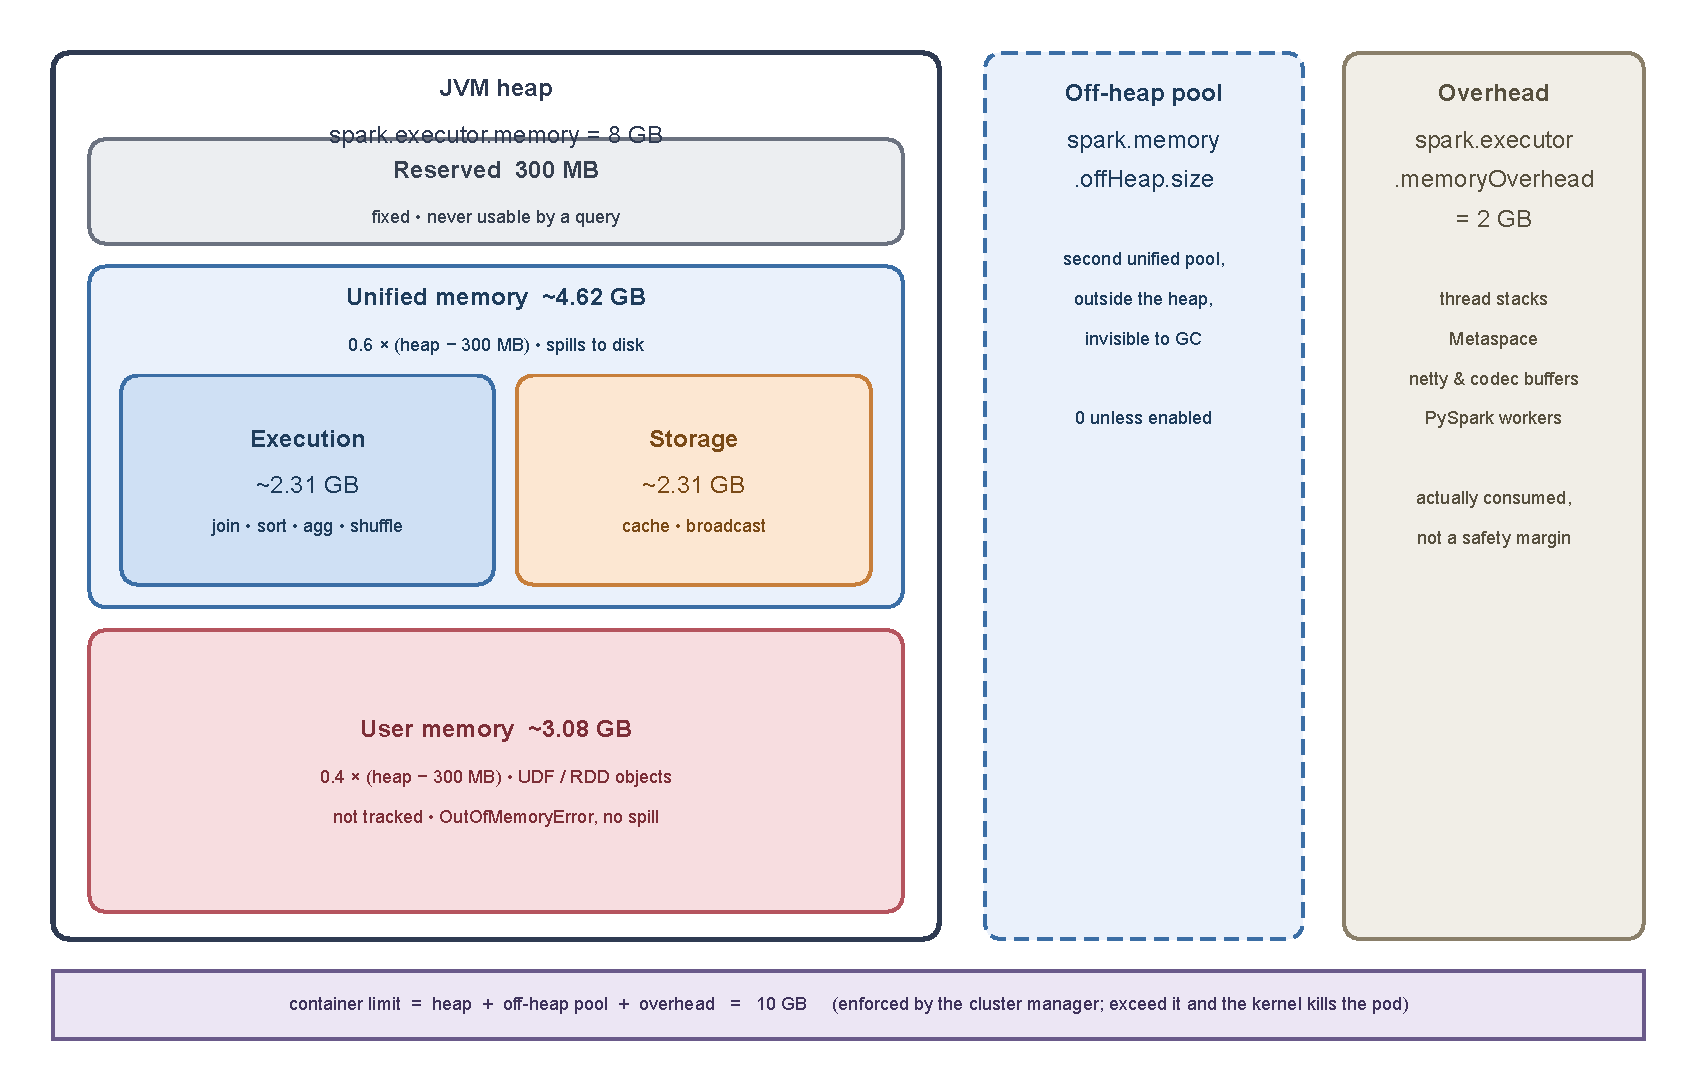
\includegraphics[width=\linewidth]{executor-memory-model.pdf}
  \caption{An executor's memory: the JVM heap (reserved / unified / user), the
  optional off-heap pool, and the overhead the process needs outside both. The
  cluster manager's container limit must cover all three. Numbers are worked for
  an 8~GB heap with 2~GB overhead.}
  \label{fig:executor-memory-model}
\end{figure}

\paragraph{Per task, not per executor.} Execution memory is shared equally across
the tasks an executor runs at once, which is \conf{spark.executor.cores}. A
larger heap with proportionally more cores gives no single task more room: memory
per task is the execution pool divided by the core count. The number of cores per
executor is therefore a memory decision as much as a parallelism one, and an
executor with too many cores spills on work a narrower one finishes in memory
(\Cref{sec:executor-sizing}).

\section{Garbage collection: Parallel, G1, ZGC}
\label{sec:mem-gc}

Because the heap is managed, the JVM must periodically find objects that are no
longer reachable and reclaim their space. This work is the \emph{garbage
collector} (GC), and for a data-processing workload it is never free: the
collector competes with the application for CPU, and some of its phases are
\emph{stop-the-world}, meaning every application thread in the JVM is frozen until
the phase completes. On an executor a long stop-the-world pause stalls every
running task at once, and if it exceeds the heartbeat timeout the driver declares
the executor lost and re-runs its work elsewhere (\Cref{sec:failure-signatures}).

Collectors differ mainly in how they trade pause length against throughput and
CPU cost.

\begin{itemize}
  \item \textbf{Parallel GC} uses multiple threads but collects the whole heap in
        one stop-the-world pause. It gives the highest raw throughput when pauses
        do not matter, but pause time grows with heap size, so a large executor
        can freeze for seconds at a time.
  \item \textbf{G1} (Garbage-First) divides the heap into equal-sized regions and
        collects a subset of them per cycle, doing most of its marking
        concurrently with the application. Pause times are shorter and roughly
        bounded regardless of heap size, at the cost of more bookkeeping and CPU.
        It is the default at the heap sizes a Spark executor typically runs and
        the collector most Spark tuning assumes.
  \item \textbf{ZGC} does essentially all of its work concurrently and keeps
        pauses under a millisecond even on very large heaps, at a higher constant
        CPU and memory overhead. It is worth choosing only for executors with
        tens of gigabytes of heap where G1 pauses are still a problem.
\end{itemize}

The generational hypothesis --- that most objects die young --- underlies all
three: they collect a small ``young'' area cheaply and often, and the full-heap
collection rarely. A workload that holds a large amount of long-lived data in
cache violates that assumption and pushes the collector toward the expensive
path, which is one more reason to cache deliberately (\Cref{ch:caching}).
Monitoring GC time is covered in \Cref{sec:reading-metrics}; the executor JVM
options that select and tune a collector are in \Cref{ch:tuning}.

\section{Serialization and its cost}
\label{sec:mem-serialization}

The engine keeps a join's hash table or a block of cached rows as one large
off-heap byte buffer rather than millions of small Java objects, which is why
that data is invisible to the garbage collector and costs nothing to collect
(\Cref{sec:mem-model}, \Cref{ch:tungsten}). Getting data into and out of that
flat form is serialization.

\emph{Serialization} is the conversion of an in-memory object graph into a flat
sequence of bytes, and \emph{deserialization} is its inverse. Spark serializes
whenever data leaves a JVM: across the network during a shuffle, to disk when
unified memory spills or a block is cached in serialized form, and when a
broadcast variable is shipped to executors. The cost is both CPU and size.

The two options for arbitrary Java objects differ sharply. The built-in Java
serializer writes the full class name and every field name and type alongside the
values, repeated for every object, so most of the output is self-description
rather than data. \emph{Kryo} writes a compact encoding --- a short numeric class
identifier and the field values --- and produces output several times smaller,
which directly reduces shuffle volume, spill size, and broadcast footprint
(\Cref{ch:tuning}).

DataFrame and SQL workloads sidestep both serializers for most operations: rows
already live in the engine's binary format (\Cref{ch:tungsten}), so moving them
is a memory copy with no object graph to walk. The Java-versus-Kryo choice still
governs RDD code, user-defined functions, and anything that puts arbitrary Java
objects into a shuffle or a broadcast --- the same user-memory objects that
\Cref{sec:mem-model} noted Spark does not manage.

\section{Summary}
\tbd

\exercisehead
\begin{exercises}
\item Given a pod memory limit and a workload description, propose
      \conf{spark.executor.memory}, \conf{spark.executor.cores}, and
      \conf{spark.executor.memoryOverhead}, and justify each number from the
      memory map in \Cref{fig:executor-memory-model}.
\end{exercises}


\part{Making Queries Fast}
\chapter{The Shuffle}
\label{ch:shuffle}

\begin{chapterintro}
Every \texttt{JOIN}, \texttt{GROUP BY}, \texttt{DISTINCT}, window function, and
repartition puts a wall between two stages: the shuffle. It writes every
partition to disk, moves it across the network, and re-reads it. It is where most
of a query's time goes. This chapter walks the write path and the read path,
shows how to size shuffle partitions from data volume instead of accepting the
default 200, and how to find and remove exchanges the query does not need.
\end{chapterintro}

\section{What a partition is: input partitions versus shuffle partitions}
\tbd

\section{The shuffle write path}
\tbd

\section{The shuffle read path}
\tbd

\section{Sizing shuffle partitions}
\tbd

\section{Shuffle compression}
\tbd

\section{Push-based shuffle}
\tbd

\section{Finding and removing unnecessary exchanges}
\tbd

\section{Summary}
\tbd

\exercisehead
\begin{exercises}
\item From a stage's shuffle-read size in the UI, compute a target partition
      count for a 128~MB task size, then verify against the observed task sizes.
\end{exercises}

\chapter{Joins}
\label{ch:joins}

\begin{chapterintro}
Spark has four ways to run a join and picks one from a size estimate. When the
estimate is right, the choice is right. When the table has no statistics ---
the common case for Iceberg, as the specimen query already showed
(\Cref{sec:catalyst-analysis}) --- the planner guesses, and a join that should
have broadcast a 30~MB dimension instead shuffles a billion rows. This chapter
covers the four strategies, how the planner chooses between them, and how to
override it when you know better than the statistics do.
\end{chapterintro}

\Cref{fig:join-strategies} shows the shape each strategy leaves in a plan. The
rest of this chapter explains why each shape exists and what it costs; the
identifiers to spot them by are catalogued in \Cref{sec:c-joins}.

\begin{figure}[htbp]
  \centering
  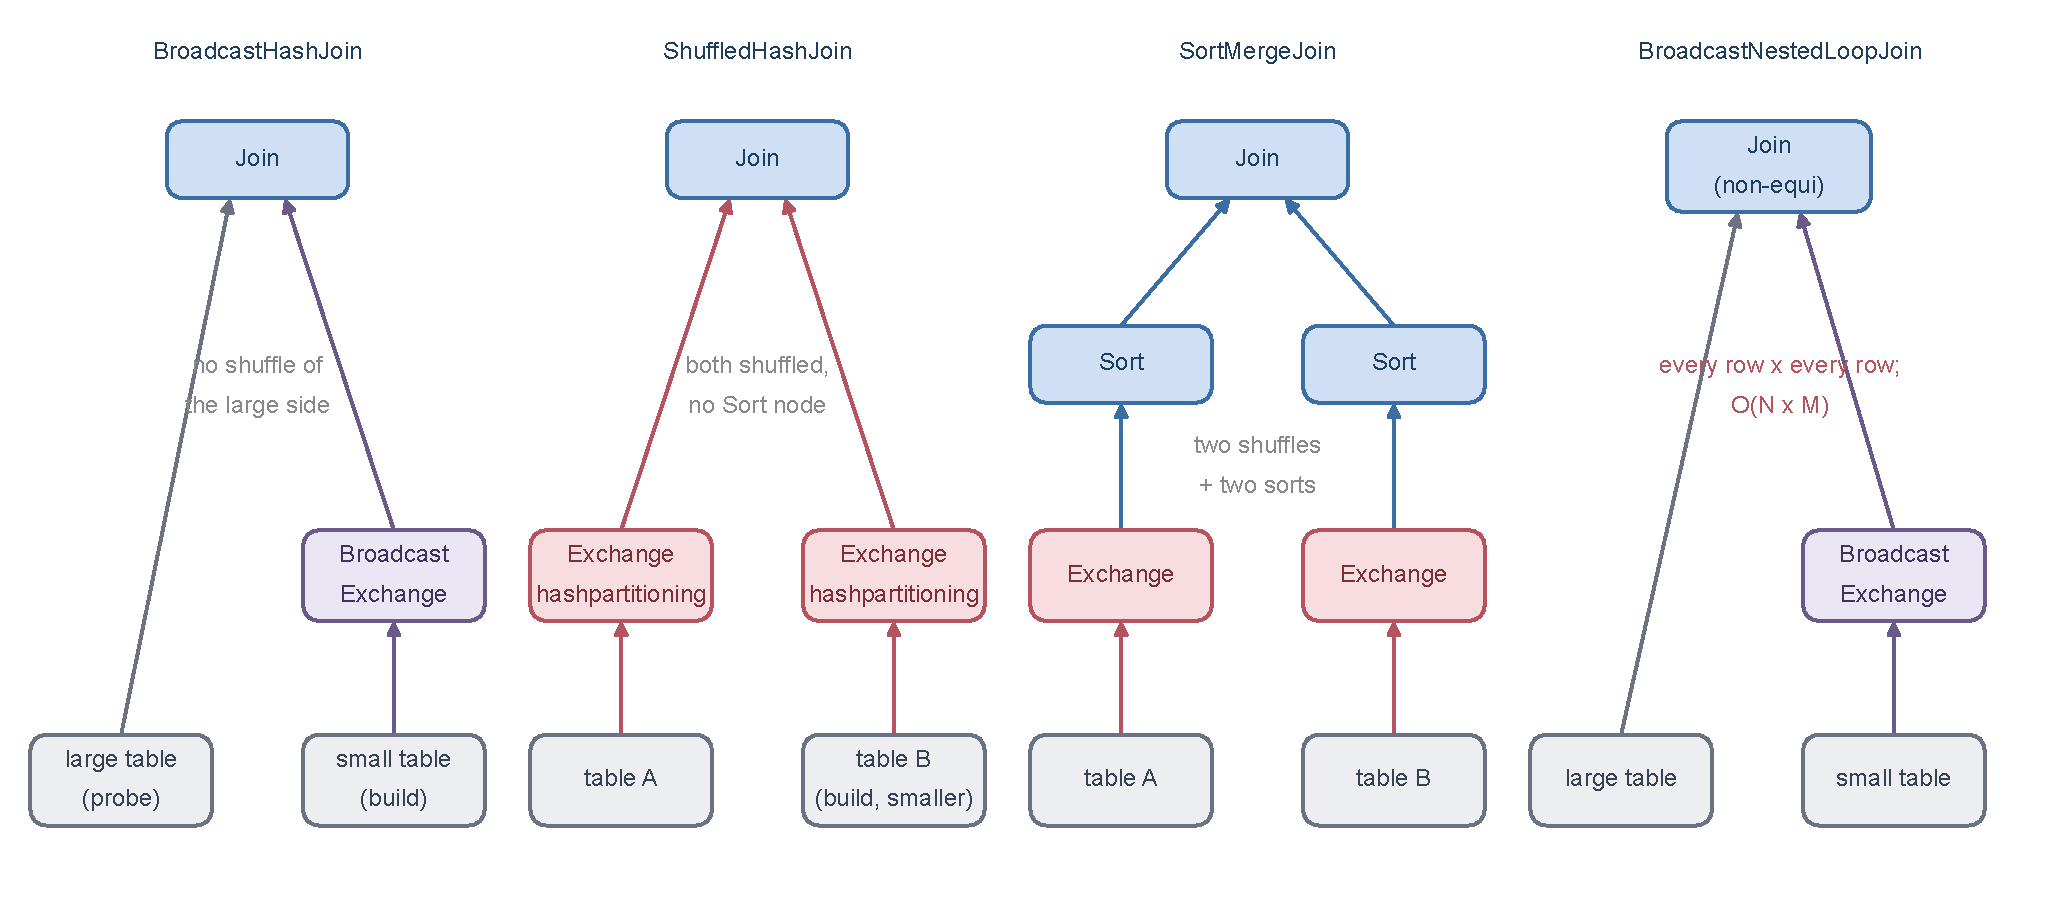
\includegraphics[width=\linewidth]{join-strategies.pdf}
  \caption{The four join strategies as plan shapes. Broadcast hash join shuffles
  nothing on the large side; shuffled hash join shuffles both sides but sorts
  neither; sort-merge join shuffles and sorts both; broadcast nested loop join
  broadcasts one side to evaluate a condition that is not an equality.}
  \label{fig:join-strategies}
\end{figure}

\section{Broadcast hash join}
\label{sec:joins-bhj}

If one side of a join is small enough, Spark skips shuffling the large side
entirely: it collects the small side to the driver, packages it once, and ships
a full copy to every executor (a \texttt{BroadcastExchange}), where it is built
into an in-memory hash table keyed on the join column. Each task on the large
side then probes that local hash table row by row --- no shuffle, no sort, and
the large side is read exactly once, in place.

This is the cheapest strategy whenever it applies, which is exactly why the
planner tries it first. Two costs are easy to underestimate. First, the
\emph{driver} holds the whole broadcast table in memory while assembling it,
at roughly twice the table's serialized size; a broadcast large enough to hurt
the driver is a self-inflicted wound distinct from anything happening on the
executors. Second, the size used to decide broadcastability is the table's
\emph{on-disk} size, and a compressed columnar file routinely decodes to
several times that once it is rows in memory (\Cref{sec:mem-heap}) --- so a
``100~MB'' table can be genuinely 500~MB--1~GB once broadcast and decoded,
which is why the planning-time threshold is conservative by design. Spark also
enforces a hard ceiling (roughly 8~GB serialized, and a few hundred million
rows) past which a table cannot be broadcast at all, regardless of the
threshold.

Put numbers on it: \texttt{dim\_product} (\Cref{sec:refenv-orders}) is a
6~MB Parquet file, comfortably under the default 10~MB
\conf{spark.sql.autoBroadcastJoinThreshold} on its real, on-disk size. Here
is what "twice the serialized size" means once that file is actually
broadcast: Parquet's columnar compression packs those 6~MB down from perhaps
20~MB of raw column values; decoded back into JVM row objects on the driver
(\Cref{sec:mem-heap}'s per-object overhead applies here too), that 6~MB file
can easily inflate to 25--35~MB in memory, and the driver holds roughly two
copies of that while it collects the file's rows and then builds the
broadcast payload to ship out --- 50--70~MB of driver heap spent
broadcasting a file whose on-disk size looked negligible. A dimension table
ten times larger inflates the same way, which is exactly why the
comfortable-looking 10~MB threshold on disk still leaves real headroom
before it threatens a driver's heap.

\section{Shuffle hash join}
\label{sec:joins-shj}

When neither side is small enough to broadcast but one side is still
meaningfully smaller than the other, Spark can shuffle both sides on the join
key and build an in-memory hash table from the smaller (build) side on each
executor, then probe it with the larger (probe) side --- without sorting
either. This is a \texttt{ShuffledHashJoin}: two shuffles, like sort-merge, but
no \texttt{Sort} nodes, which makes it cheaper than sort-merge whenever the
build side reliably fits in memory per partition.

That condition is also its weakness: unlike sort-merge, a shuffled hash join
has no graceful way to spill an oversized build-side partition to disk. If a
single partition's build side is larger than expected --- most often because of
skew --- the task fails outright rather than slowing down. Spark's planner is
correspondingly conservative about choosing it: by default it prefers
sort-merge whenever both sides have sortable keys
(\conf{spark.sql.join.preferSortMergeJoin}\,=\,\texttt{true}), and only
considers a shuffled hash join when that preference is turned off and the
build side is estimated at at least three times smaller than the probe side.
Concretely: with the preference off, an estimated 500~MB \texttt{dim\_customer}
against a 2~GB \texttt{orders} slice qualifies (2~GB is $4\times$ larger), and
the plan shows \texttt{ShuffledHashJoin} with no \texttt{Sort} node on either
input; the same 500~MB against only 1~GB of \texttt{orders} does not qualify
($2\times$, short of the $3\times$ bar), and the planner falls back to
sort-merge instead, adding a \texttt{Sort} node to each side of the plan that
was absent in the qualifying case.

\section{Sort-merge join}
\label{sec:joins-smj}

Sort-merge join is the default for two large, roughly comparable inputs, and it
is what the specimen query uses in \Cref{ch:catalyst}: both sides are shuffled
on the join key, each partition is then sorted locally, and the join is
produced by walking both sorted streams together, advancing whichever key is
behind. It is the most expensive of the equi-join strategies --- two shuffles
and two sorts --- but it is also the most robust: a sort spills to disk cleanly
under memory pressure the way a hash table cannot, so it scales to inputs of any
size on either side.

\section{Broadcast nested loop join}
\label{sec:joins-bnlj}

An equi-join needs a hash or a sort; a join whose condition is not an equality
--- \texttt{ON o.order\_total > c.credit\_limit}, for instance --- needs neither, and
Spark falls back to comparing every row of one side against every row of the
other. If one side is small enough to broadcast, this is a
\texttt{BroadcastNestedLoopJoin}: no shuffle, but $O(N \times M)$ comparisons
inside each task. If neither side is small enough to broadcast, Spark falls all
the way back to a \texttt{CartesianProduct} (\Cref{sec:c-joins}), which is
rarely what you want on two large tables and is usually a sign that a join
condition is missing.

\begin{note}
A full outer join cannot use broadcast hash join, even with an explicit hint:
there is no way to detect an unmatched row on the broadcast side without
scanning it, which the strategy is built to avoid. A \texttt{FULL OUTER} join
falls back to sort-merge regardless of size.
\end{note}

\section{How the planner chooses}
\label{sec:joins-selection}

For an equi-join, the planner tries strategies in a fixed order, stopping at
the first one that applies:

\begin{enumerate}
  \item an explicit join hint, if the query has one (\Cref{sec:joins-forcing});
  \item \textbf{broadcast hash join}, if either side's estimated size is at or
        below \conf{spark.sql.autoBroadcastJoinThreshold} (10~MB by default);
  \item \textbf{sort-merge join}, if \conf{spark.sql.join.preferSortMergeJoin}
        is \texttt{true} (the default) and the keys are sortable;
  \item \textbf{shuffled hash join}, if that preference is off and the build
        side is estimated at least $3\times$ smaller than the probe side and
        fits per-partition memory;
  \item \textbf{sort-merge join}, as the fallback for any remaining equi-join
        with sortable keys.
\end{enumerate}

Every one of these decisions, except the explicit hint, is made from
\emph{estimated} sizes --- from the catalog if statistics exist, or from
on-disk file size if they do not (\Cref{sec:catalyst-analysis}). This is the
single most common way real joins go wrong: not a bug, but a plan built on a
wrong number.

Trace one query through the ordered list to see how the choice actually
falls out. For \texttt{orders JOIN dim\_customer}, with
\texttt{dim\_customer} estimated at 500~MB and no hint present: step~1 does
not apply (no hint); step~2 does not apply (500~MB is far past the 10~MB
threshold); step~3 \emph{does} apply --- \conf{preferSortMergeJoin} is
\texttt{true} by default and both join keys are plain strings, sortable ---
so the planner stops right there and emits a sort-merge join. Step~4 (the
shuffled-hash-join check) is never even evaluated, because the search stops
at the first rule that matches; a shuffled hash join only becomes reachable
at all if someone first turns \conf{preferSortMergeJoin} off, which is why
\Cref{sec:joins-shj} described it as the strategy the planner reaches for
last, not by default.

\section{Forcing a strategy}
\label{sec:joins-forcing}

When the estimate is missing or wrong, a hint overrides it directly:

\begin{lstlisting}[language=SQL,caption={Forcing a broadcast when statistics are missing},captionpos=b]
SELECT /*+ BROADCAST(p) */ o.product_id, p.category
FROM orders o JOIN dim_product p ON o.product_id = p.product_id;
\end{lstlisting}

The hints, in priority order, are \texttt{BROADCAST} (or
\texttt{BROADCASTJOIN}/\texttt{MAPJOIN}), \texttt{SHUFFLE\_MERGE} (or
\texttt{MERGE}) for sort-merge, and \texttt{SHUFFLE\_HASH} for a shuffled hash
join. A hint is an instruction, not a suggestion: Spark will honor it even when
its own estimate disagrees, so a stale hint on a table that has since grown
past a sane broadcast size is a real production hazard, not a theoretical one.

The more durable fix is to give the planner real numbers instead of overriding
its guess:

\begin{lstlisting}[language=SQL,caption={Giving the CBO real statistics},captionpos=b]
ANALYZE TABLE db.dim_product COMPUTE STATISTICS FOR ALL COLUMNS;
\end{lstlisting}

Iceberg tables carry file-level size and row counts in their metadata for free,
but not the column-level statistics the cost-based optimizer uses to size a
join --- which is exactly why the specimen query's small \texttt{dim\_product}
table was shuffled instead of broadcast in \Cref{ch:catalyst}. Running
\texttt{ANALYZE} once after a table's data changes materially is usually
cheaper, and safer over time, than hard-coding a hint.

\begin{tip}
Adaptive Query Execution catches many of these mistakes without any of the
above: it re-evaluates a join's strategy \emph{after} its inputs have shuffled,
against their real post-shuffle size, and promotes a sort-merge join to a
broadcast if the data turns out small enough (\Cref{ch:aqe}). Hints and
\texttt{ANALYZE} matter most for the joins AQE cannot rescue --- most often
because the small side is broadcastable only before a shuffle changes its
size, not after.
\end{tip}

\section{Storage-partitioned joins for bucketed Iceberg tables}
\label{sec:joins-spj}

Every strategy above pays the same structural cost sort-merge join pays most
visibly: two shuffles, one per side, every single time the query runs, even
though the join key never changes between runs. The next strategy exists to
avoid paying that cost at query time at all, by doing the equivalent work
once, up front, when the tables are written. Every strategy above assumes
the two sides arrive unaligned and have to be shuffled into agreement. If both tables are already \emph{bucketed} on the join
key with the same bucket count (\Cref{ch:iceberg-layout}), that assumption is
false: rows that must be compared are already co-located file by file, and
Spark can join corresponding buckets directly with no exchange on either
side --- a \emph{storage-partitioned join}. This turns the most expensive part
of a sort-merge join, the two shuffles, into work done once at write time
instead of on every query that joins the tables.

The condition is strict: both tables need the identical bucket transform and
bucket count on the join column, and Spark needs
\conf{spark.sql.sources.v2.bucketing.enabled} set to consider it at all. It is
a design decision made when the tables are created, not a query-time tuning
knob --- worth it specifically for a join pattern repeated often enough that
paying the shuffle cost once, at write time, beats paying it on every read.

\section{Summary}
\label{sec:joins-summary}

Four strategies, in the order the planner tries them: broadcast hash join
(cheapest, but bounded by the small side's real decoded size, not its file
size), sort-merge join (the robust default for two large sides), shuffled hash
join (cheaper than sort-merge when it applies, but unable to spill), and
broadcast nested loop or Cartesian for a non-equi condition. Every automatic
choice rests on a size estimate, and Iceberg tables commonly lack the
column statistics that estimate needs --- \texttt{ANALYZE TABLE} and join hints
exist specifically to correct that, and AQE corrects a real subset of it for
free at runtime. Bucketing both sides of a frequent join on the same key
removes the shuffle from the decision entirely.

\exercisehead
\begin{exercises}
\item Given four table sizes and the broadcast threshold, predict each join's
      strategy. Then change one config value and predict which join flips.
\item Run the specimen query, then run \texttt{ANALYZE TABLE dim\_product
      COMPUTE STATISTICS FOR ALL COLUMNS} and run it again. Did the join
      strategy change? Explain from \Cref{sec:joins-selection}.
\item Write a join with a non-equi condition on two tables, neither of which is
      small. Confirm in \texttt{EXPLAIN FORMATTED} that it becomes a
      \texttt{CartesianProduct}, and rewrite it to avoid one.
\end{exercises}

\chapter{Adaptive Query Execution}
\label{ch:aqe}

\begin{chapterintro}
The Catalyst optimizer plans before it has seen any data. Adaptive Query
Execution re-plans after each shuffle, when the real partition sizes are known.
It coalesces hundreds of tiny partitions into a few good ones, promotes a
sort-merge join to a broadcast when the shuffled side turns out small, and splits
a skewed partition so one task stops holding up the stage. This chapter covers
what AQE re-decides, from what evidence, and which planning-time decisions it can
still override.
\end{chapterintro}

\section{Why runtime beats planning time}
\tbd

\section{Coalescing shuffle partitions}
\tbd

\section{Converting sort-merge to broadcast at runtime}
\tbd

\section{The two broadcast thresholds}
\tbd

\section{Skew-join handling: split and replicate}
\tbd

\section{\texttt{parallelismFirst} and partition count}
\tbd

\section{Reading an AQE plan}
\tbd

\section{Summary}
\tbd

\exercisehead
\begin{exercises}
\item Disable AQE and run a skewed join; record the straggler task. Re-enable it
      and compare the plan and the task-time distribution.
\end{exercises}

\chapter{Partitioning, Bucketing, and Pruning}
\label{ch:pruning}

\begin{chapterintro}
The cheapest data to move is data you never read. Partition pruning skips whole
directories; dynamic partition pruning does it using values discovered from the
other side of a join; bucketing lays data out so a join needs no shuffle at all.
Each of these is easy to defeat --- a function on the partition column, a
\texttt{CAST}, a stray \texttt{SELECT *} --- and the plan tells you when you
have. This chapter covers each mechanism and how to confirm it is working.
\end{chapterintro}

\section{Partition pruning and the pushdown killers}
\tbd

\section{Dynamic partition pruning}
\tbd

\section{Bucketing to avoid a shuffle}
\tbd

\section{\texttt{repartition} versus \texttt{coalesce}}
\label{sec:repartition-coalesce}
\tbd

\section{Column pruning and \texttt{ReadSchema}}
\tbd

\section{Summary}
\tbd

\exercisehead
\begin{exercises}
\item Write the same filter three ways --- a function on the partition column, a
      \texttt{CAST}, and a plain literal --- and check which keeps
      \texttt{PartitionFilters} populated in the scan node.
\end{exercises}

\chapter{Caching and Reuse}
\label{ch:caching}

\begin{chapterintro}
Caching keeps a result Spark would otherwise recompute --- but the wrong cache
wastes storage memory and starves execution, and a cache used once is pure
overhead. Spark also reuses work you did not ask it to: an identical exchange or
subquery computed once and read twice. This chapter covers when caching pays,
which storage level to pick against the GC budget from \Cref{ch:execmem}, and how
to see reuse in a plan. It is also where execution and storage memory finally
meet at runtime.
\end{chapterintro}

\section{When caching pays}
\tbd

\section{Lazy \texttt{cache()} versus eager \texttt{CACHE TABLE}}
\tbd

\section{Storage levels and the GC trade-off}
\tbd

\section{How execution and storage memory borrow at runtime}
\tbd

\section{Exchange and subquery reuse}
\tbd

\section{Unpersist and cache thrashing}
\tbd

\section{Summary}
\tbd

\exercisehead
\begin{exercises}
\item Build a query that reads one CTE twice. Show the plan reusing the exchange,
      then change the query so the reuse breaks and measure the difference.
\end{exercises}


\part{The Iceberg Lakehouse}
\chapter{Table Formats and the Iceberg Spec}
\label{ch:iceberg-spec}

\begin{chapterintro}
An Iceberg table is not a directory of Parquet files with a manifest bolted on.
It is a tree: a catalog pointer to a metadata file, to a manifest list, to
manifests, to data and delete files --- every level immutable, every commit a
single atomic pointer swap. Reads consult this tree before touching any data.
This chapter walks the spec (format version 2) against a real table's metadata
tables so you can draw the tree from memory.
\end{chapterintro}

\section{From Hive tables to table formats}
\tbd

\section{The Iceberg spec, format version 2}
\tbd

\section{Snapshots and the metadata tree}
\tbd

\section{Position deletes versus equality deletes}
\tbd

\section{Iceberg, Delta Lake, and Hudi}
\tbd

\section{Summary}
\tbd

\exercisehead
\begin{exercises}
\item Commit three appends to a table, then inspect \texttt{metadata\_log\_entries},
      \texttt{snapshots}, and \texttt{manifests}. Explain how many metadata files
      and manifests exist and why.
\end{exercises}

\chapter{Catalogs and Commits}
\label{ch:catalogs}

\begin{chapterintro}
The catalog is the one component that turns a table name into the location of its
current metadata --- and the point at which a commit becomes atomic. Writing new
metadata is not a commit until the catalog's pointer is swapped to it. When two
writers race, one wins the swap and the other retries. This chapter covers what
the Hive Metastore and REST catalogs do, how the atomic swap works, and how to
tune retries so a busy table does not fail commits under contention.
\end{chapterintro}

\section{What a catalog does}
\tbd

\section{The Hive Metastore catalog}
\tbd

\section{The REST catalog}
\tbd

\section{The atomic pointer swap}
\tbd

\section{Optimistic concurrency and retries}
\tbd

\section{Catalog configuration in Spark}
\tbd

\section{Summary}
\tbd

\exercisehead
\begin{exercises}
\item Run two writers into the same table. Observe the retry, then find the
      winning and losing commit attempts in the snapshot log.
\end{exercises}

\chapter{Iceberg Partitioning and Layout}
\label{ch:iceberg-layout}

\begin{chapterintro}
Iceberg partitioning is hidden: you filter on \texttt{event\_ts} and Iceberg
derives the predicate on \texttt{day(event\_ts)} for you, so a query never
references a partition column directly and pruning does not break when the
scheme changes. This chapter covers the partition transforms, evolving a spec
without rewriting history, sort orders and Z-ordering, target file size, and the
write-distribution mode --- the choices that decide how much a reader and a
writer have to move.
\end{chapterintro}

\section{Hidden partitioning and partition transforms}
\label{sec:ice-partitioning}

A classic Hive table's partition column is a real column duplicated into the
directory path --- a query has to filter on that exact derived value
(\texttt{WHERE event\_date = '2026-09-20'}) for pruning to fire, and a filter
on the underlying timestamp (\texttt{WHERE event\_ts >= \ldots}) does not
automatically resolve to it. Iceberg's partition spec instead names a
\emph{transform} of a source column --- \texttt{day(event\_ts)},
\texttt{bucket(16, route\_id)}, \texttt{truncate(4, zone)} --- and stores the
computed value in the manifest, not as a queryable column at all. The planner
derives the partition predicate from a filter on the source column itself, so
the specimen query's plain \texttt{event\_ts >= TIMESTAMP '\ldots'} filter
from \Cref{sec:pruning-static} prunes correctly with no partition column ever
appearing in the query text.

\Cref{tab:ice-transforms} covers the transforms this stack uses.

\begin{table}[htbp]
\centering
\caption{Common Iceberg partition transforms}
\label{tab:ice-transforms}
\begin{tabular}{@{}llp{5.2cm}@{}}
\toprule
\textbf{Transform} & \textbf{Use case} & \textbf{Notes} \\
\midrule
\texttt{day} / \texttt{hour} & Time-series data filtered by a timestamp range &
  Coarser (\texttt{day}) means fewer, larger partitions; \texttt{hour} suits
  high-volume streams (\Cref{ch:streaming}) \\
\texttt{bucket(n, col)} & High-cardinality key with equality or join
  predicates & Even file distribution by hash; enables storage-partitioned
  joins (\Cref{sec:joins-spj}) when both sides share the spec \\
\texttt{truncate(n, col)} & String or numeric prefix filters & Groups by a
  value prefix without one partition per distinct value \\
\texttt{identity} & Low-cardinality column filtered directly & Same as
  classic partitioning, just recorded the hidden way \\
\bottomrule
\end{tabular}
\end{table}

\begin{tip}
Prefer \texttt{day} over \texttt{identity} on a raw timestamp: an
\texttt{identity} partition on \texttt{event\_ts} would create one partition
\emph{per distinct timestamp value}, which is not partitioning at all --- it is
one file per row's worth of metadata. Always partition on a transform coarse
enough to group many rows per partition.
\end{tip}

\section{Partition evolution}
\label{sec:ice-partition-evolution}

A classic Hive table's partitioning is fixed at creation; changing it means
rewriting every file under the new scheme. Iceberg's partition spec can
change (\texttt{ALTER TABLE \ldots ADD PARTITION FIELD}) without touching a
single existing file, because the transform that produced a file's partition
value is recorded per-manifest, not assumed globally --- old manifests keep
describing old files under the old spec, new manifests describe new files
under the new spec, and a query spans both by evaluating each manifest
against its own recorded spec.

This is why moving from \texttt{month(event\_ts)} to \texttt{day(event\_ts)}
as a table grows is a metadata-only operation, not a maintenance project: new
data lands under the finer scheme immediately, old data keeps the coarser
scheme it was written with, and a query filtering by date prunes correctly
against both --- coarser pruning on the old partitions, finer pruning on the
new ones, with no explicit migration step and no downtime.

\section{Sort orders and Z-ordering}
\label{sec:ice-sort-order}

A partition spec controls which \emph{files} a filter can skip; a
\emph{sort order} controls how much of the \emph{content} within a kept file
can still be skipped, via the column min/max statistics
\Cref{ch:iceberg-spec}'s manifests already carry per file. Files written
sorted by a column have tight, non-overlapping min/max ranges across files ---
a filter on that column can then skip whole files even within one partition,
the same statistics-based pruning \Cref{sec:c-pushdown} described for row
groups, just at the file level.

A single sort order only helps predicates on the columns it is sorted by,
front to back. \emph{Z-ordering} (\texttt{rewrite\_data\_files} with
\texttt{sort\_order} type \texttt{zorder}) interleaves the bits of several
columns into one sort key instead, trading perfect single-column ordering for
imperfect-but-useful ordering on every column in the set simultaneously ---
the right choice when queries filter on different columns unpredictably
rather than one column consistently.

\section{Target file size and the small-files problem}
\label{sec:ice-file-size}

Every file a reader opens costs a fixed overhead --- opening the file, reading
its footer, resolving its schema --- independent of how many rows it holds
(\Cref{sec:shape-jobs}'s input-partition sizing runs into the same fixed cost
from the other direction). A table accumulating many small files, typically
from frequent low-volume commits (a streaming job flushing every micro-batch,
\Cref{ch:streaming}), pays that overhead over and over for little data each
time. \texttt{write.target-file-size-bytes} (512~MB by default) sets what a
write aims for; \Cref{ch:iceberg-write}'s compaction procedures are the
after-the-fact fix for files that already landed too small.

\section{Write distribution modes}
\label{sec:ice-write-distribution}

Before a write's rows are grouped into per-partition files, Spark may need to
shuffle them so that all rows for a given partition value land together
rather than scattered across every task's output --- exactly the shuffle
mechanics from \Cref{ch:shuffle}, applied to a write instead of a read.
\texttt{write.distribution-mode} chooses how:

\begin{description}
  \item[\texttt{none}] writes rows in whatever order the upstream plan already
        produced them, with no shuffle. Cheapest, but every task can touch
        every partition, so a table with many partitions ends up with many
        small files per commit --- one per (task, partition) pair touched.
  \item[\texttt{hash}] (the default for unpartitioned or partitioned tables
        with a defined spec) shuffles by partition value first, so each task
        after the shuffle owns one partition's rows and writes one file for
        it. This is the direct fix for the \texttt{none} mode's small-files
        problem, at the cost of the shuffle itself.
  \item[\texttt{range}] shuffles by a sampled range of the sort order instead
        of a hash, producing files with tighter, non-overlapping value
        ranges --- the write-time complement to \Cref{sec:ice-sort-order}'s
        pruning benefit, at a higher planning cost (a sampling pass before
        the real shuffle).
\end{description}

\section{Summary}
\label{sec:ice-layout-summary}

Iceberg partitioning is hidden behind a transform of a source column, so
pruning works from a plain filter on that column with no partition column in
the query; \texttt{day}/\texttt{hour} suit time-series filters,
\texttt{bucket} suits high-cardinality keys and storage-partitioned joins,
and an \texttt{identity} transform on a high-cardinality column is a
modeling mistake, not a partitioning choice. Evolving the spec is
metadata-only because old files keep the spec they were written under. A
sort order or Z-order tightens the per-file statistics that let a reader
skip whole files inside a kept partition; target file size and the write
distribution mode are what decide whether a write produces a few
well-sized files or many small ones in the first place.

\exercisehead
\begin{exercises}
\item Given a daily data volume and a query pattern, choose a partition spec.
      Justify it against the target of 128~MB--1~GB per partition per write.
\item Evolve a table's partition spec from \texttt{month(event\_ts)} to
      \texttt{day(event\_ts)}. Confirm from the \texttt{partitions} metadata
      table that old and new data report different specs.
\item Write the same DataFrame with \texttt{write.distribution-mode} set to
      \texttt{none} and then \texttt{hash}. Compare the file count per
      partition in each case.
\end{exercises}

\chapter{Reading Iceberg Efficiently}
\label{ch:iceberg-read}

\begin{chapterintro}
Before the Iceberg reader opens a single data file, it has already skipped most
of them --- by partition, by manifest, by column statistics, and optionally by
bloom filter. Each layer needs the query's filter in a form it understands, and
the scan report tells you how well each one worked. This chapter covers the
pruning layers, the metrics modes that feed them, and how to read a scan report
as a diagnostic.
\end{chapterintro}

\section{Manifest pruning and metadata filtering}
\tbd

\section{Column statistics and predicate pushdown into Iceberg}
\tbd

\section{Metrics modes: \texttt{full}, \texttt{truncate}, \texttt{counts}, \texttt{none}}
\tbd

\section{Bloom filters}
\tbd

\section{Vectorized reads}
\tbd

\section{Split planning}
\tbd

\section{The metadata tables as a diagnostic}
\tbd

\section{Summary}
\tbd

\exercisehead
\begin{exercises}
\item Run a selective query and, from the scan report, compute the fraction of
      data pruned at each layer (partition, manifest, file).
\end{exercises}

\chapter{Writing and Maintaining Iceberg}
\label{ch:iceberg-write}

\begin{chapterintro}
Copy-on-write rewrites whole files on every update: slow writes, fast reads.
Merge-on-read writes small delete files instead: fast writes, slower reads until
compaction catches up. The choice is a function of your update rate and your read
latency budget, and it commits you to a maintenance schedule --- compaction,
snapshot expiration, orphan-file cleanup --- in a specific order. This chapter
covers the write modes, optimizing \texttt{MERGE}, and running maintenance
without deleting data a reader still needs.
\end{chapterintro}

\section{Copy-on-write versus merge-on-read}
\tbd

\section{\texttt{MERGE}, \texttt{UPDATE}, and \texttt{DELETE}}
\tbd

\section{Write distribution and skew on write}
\tbd

\section{Compacting data files}
\tbd

\section{Rewriting manifests}
\tbd

\section{Snapshot expiration and orphan files}
\tbd

\section{Metadata management for streaming tables}
\tbd

\section{Summary}
\tbd

\exercisehead
\begin{exercises}
\item Run a \texttt{MERGE} with and without the partition column in the
      \texttt{ON} clause. Explain the difference in files scanned from the plan.
\end{exercises}


\part{Operating Spark}
\chapter{Tuning Resources and Configuration}
\label{ch:tuning}

\begin{chapterintro}
This chapter does not hand you a table of recommended settings. It derives an
executor shape from the memory map in \Cref{ch:execmem} and the shuffle in
\Cref{ch:shuffle}, so that every number --- cores, heap, overhead, partition
count --- has a reason you can defend. It then covers dynamic allocation, the
external shuffle service on Kubernetes, configuration precedence, and running
Spark behind Kyuubi for many users. For the standalone list of tuning knobs with
values, see \texttt{spark\_memory\_tuning.md} in the repository root.
\end{chapterintro}

\section{Executor sizing from the mechanism}
\label{sec:executor-sizing}
\tbd

\section{Dynamic allocation}
\label{sec:dynamic-allocation}
\tbd

\section{Parallelism defaults}
\tbd

\section{The external and push-based shuffle service}
\tbd

\section{Configuration precedence and profiles}
\tbd

\section{Kyuubi and multi-tenancy}
\tbd

\section{Summary}
\tbd

\exercisehead
\begin{exercises}
\item Take a job that spills. Propose two different fixes --- more memory versus
      fewer cores --- and predict which the mechanism favours, and why.
\end{exercises}

\chapter{Debugging and Profiling}
\label{ch:debugging}

\begin{chapterintro}
A slow job leaves evidence: in the SQL tab, the stages tab, the executor
metrics, the event log, and --- when you need it --- a flame graph. This chapter
teaches you to read that evidence in order, so that "the job is slow" becomes
"stage 4 is skewed" or "the executors are GC-bound" in a few minutes. It also
catalogs the failure signatures --- OOM and container kills, fetch failures,
stragglers --- and what each looks like before you reach for a fix.
\end{chapterintro}

\section{The Spark UI as a diagnostic}
\tbd

\section{Event logs and the history server}
\tbd

\section{Reading task, shuffle, spill, and GC metrics}
\label{sec:reading-metrics}
\tbd

\section{Common failure signatures}
\label{sec:failure-signatures}
\tbd

\section{async-profiler and flame graphs}
\tbd

\section{Debugging query plans}
\tbd

\section{Summary}
\tbd

\exercisehead
\begin{exercises}
\item Given three anonymized stage summaries, diagnose each as skew,
      under-partitioned, or GC-bound, and name the evidence.
\end{exercises}

\chapter{Streaming into the Lakehouse}
\label{ch:streaming}

\begin{chapterintro}
Structured Streaming is the same query engine over an unbounded table, processing
one micro-batch at a time and ending each batch with a single Iceberg commit. The
whole model from the earlier parts still applies --- the shuffle, the executor
budget, the commit --- but with two new pressures: state that must be kept
between batches, and a commit cadence that produces small files faster than a
batch job. This chapter covers the streaming model and what it does to an Iceberg
table.
\end{chapterintro}

\section{The micro-batch model and the unbounded table}
\tbd

\section{Sources and sinks}
\tbd

\section{Event time and watermarking}
\tbd

\section{Stateful operations and the state store}
\tbd

\section{Output modes and triggers}
\tbd

\section{Exactly-once and the commit}
\tbd

\section{Writing to Iceberg: cadence, small files, maintenance}
\tbd

\section{Summary}
\tbd

\exercisehead
\begin{exercises}
\item Given a trigger interval and an input rate, estimate files committed per
      hour and the compaction cadence needed to keep the table healthy.
\end{exercises}


\part{Internals}
\chapter{Tungsten and Code Generation}
\label{ch:tungsten}

\begin{chapterintro}
Below the plan, a stage does not interpret operators row by row. Tungsten stores
rows as packed off-heap bytes, and whole-stage code generation collapses an
operator subtree into a single generated Java method that the JIT compiles to
tight machine code. This chapter opens that layer: the binary row format,
off-heap memory management, cache-aware computation, and the generated code you
can actually read with \texttt{EXPLAIN CODEGEN}.
\end{chapterintro}

\section{The Tungsten binary row format}
\tbd

\section{Off-heap memory management}
\tbd

\section{Cache-aware computation}
\tbd

\section{Whole-stage code generation internals}
\tbd

\section{Expression code generation}
\tbd

\section{Columnar processing and vectorization}
\tbd

\section{Summary}
\tbd

\exercisehead
\begin{exercises}
\item Run \texttt{EXPLAIN CODEGEN} on a filter-and-project query. Identify which
      operators were fused into one generated method and which were not.
\end{exercises}

\chapter{The Shuffle Framework and the Scheduler}
\label{ch:scheduler}

\begin{chapterintro}
\Cref{ch:shuffle} treated the shuffle as a wall. This chapter builds the wall:
the shuffle manager and its writers, the map output tracker that tells reduce
tasks where to fetch from, the DAG scheduler that cuts a plan into stages, the
task scheduler that places tasks on executors, and the block transfer service
that moves the bytes. It is the machinery behind every stage boundary and every
straggler.
\end{chapterintro}

\section{The shuffle manager and shuffle writers}
\label{sec:sched-shuffle-manager}

Every shuffle on a modern Spark version goes through \texttt{SortShuffleManager}
--- the separate hash-based shuffle manager from early Spark versions was
removed once sort-based shuffle's one-file-plus-index-per-task layout
(\Cref{sec:shuffle-write}) proved strictly better at scale. What varies is
which \emph{writer} a given shuffle uses underneath that one manager, chosen
automatically from the shuffle's own properties:

\begin{description}
  \item[\texttt{BypassMergeSortShuffleWriter}] fires when the shuffle has no
        map-side aggregation and the partition count is below
        \conf{spark.shuffle.sort.bypassMergeThreshold} (200 by default) ---
        cheap enough, at that few partitions, to just write one file per
        partition directly and concatenate them, skipping the sort step
        entirely.
  \item[\texttt{UnsafeShuffleWriter}] (the "serialized" path) fires when the
        serializer supports relocating serialized values without
        deserializing them (Kryo does, under most configurations) and there
        is no map-side aggregation --- it sorts the same compact
        \emph{(partition-id, pointer)} arrays \Cref{sec:tungsten-cache-aware}
        described, spilling and merging already-serialized bytes with no
        object ever reconstructed mid-sort.
  \item[\texttt{SortShuffleWriter}] is the general fallback --- a real
        record-by-record sort by partition (and key, if the shuffle
        aggregates) --- used whenever the other two writers' preconditions
        do not hold, at correspondingly higher cost.
\end{description}

The upshot: a shuffle you did not particularly optimize is not necessarily
running the expensive general path --- Spark already picks the cheapest
writer whose preconditions hold for that specific shuffle.

\section{The map output tracker}
\label{sec:sched-map-output-tracker}

A reduce task needs to know which executors hold which map task's output
before it can fetch anything --- that registry is the \emph{map output
tracker}. The driver's copy, \texttt{MapOutputTrackerMaster}, is the single
authoritative record, updated every time a map task finishes (with its
output location) and every time an executor is lost (with that executor's
outputs invalidated, which is precisely the trigger behind
\Cref{sec:failure-signatures}'s stage-resubmission behavior). Executors hold
a read-only, periodically-refreshed cache of the same information,
\texttt{MapOutputTrackerWorker}, so that a reduce task can resolve fetch
locations locally most of the time without an RPC to the driver for every
single task.

\section{The DAG scheduler and the task scheduler}
\label{sec:sched-dag-task}

Two schedulers do two different jobs, one layered on top of the other. The
\textbf{DAG scheduler} operates on RDD lineage: it walks the dependency
graph backward from an action, cutting a new stage boundary at every wide
dependency (\Cref{sec:shape-deps}), and submits stages to run only
once their upstream stages have finished --- this is the component that
turns one query into the job/stage structure \Cref{ch:shape} first
introduced, and the one that decides, on a \texttt{FetchFailedException},
exactly which upstream stage needs to re-run. The \textbf{task scheduler}
(\texttt{TaskSchedulerImpl}) operates one level down, inside an already-submitted
stage: given a set of runnable tasks and the current executors, it decides
\emph{which} task runs on \emph{which} executor, honoring the locality
preferences below and retrying a task, up to
\conf{spark.task.maxFailures}, on the executor it failed on before giving
up on that executor for that task.

\section{RPC and block transfer}
\label{sec:sched-rpc-transfer}

Coordination messages (task assignment, status updates, the map output
tracker's queries) travel over Spark's internal RPC layer, built on Netty;
the actual shuffle bytes travel over a separate path, the
\texttt{NettyBlockTransferService}, which is what a reduce task's fetch
request and an executor's block-serving response both ultimately go
through --- the same service the external shuffle service
(\Cref{sec:shuffle-external}) reimplements as a standalone process, so that
block-serving keeps working with no executor JVM behind it at all.

\section{Locality and speculation}
\label{sec:sched-locality-speculation}

Placing a task on the executor that already holds its input data avoids a
network read entirely; the task scheduler ranks candidate executors by
locality level --- \texttt{PROCESS\_LOCAL} (same JVM), \texttt{NODE\_LOCAL}
(same node, different executor), \texttt{RACK\_LOCAL}, then \texttt{ANY} ---
and will wait briefly (\conf{spark.locality.wait}, 3s by default) for a
better-locality slot to free up before falling back to a worse one. On this
stack's typical setup (compute and storage separated, GCS rather than
co-located HDFS), locality beyond \texttt{ANY} rarely applies to the initial
read regardless of this waiting, since there is no node the data is
particularly local to; it still matters for shuffle reads, where a task
scheduled on the same node as (some of) its shuffle input avoids that
portion of the network transfer.

Speculation (\Cref{sec:failure-signatures}) is the task scheduler's own
mechanism for the case locality cannot fix: once a task has run past
\conf{spark.speculation.multiplier} times the median duration for its stage,
the scheduler launches a second, speculative copy on a different executor
and accepts whichever attempt's result lands first, discarding the other ---
a scheduling-level decision independent of the DAG scheduler's stage-level
view, since a straggler is a single task problem, not a stage problem.

\section{Summary}
\label{sec:sched-summary}

One shuffle manager, three writers chosen by preconditions rather than
configuration you set directly: bypass for few partitions, serialized-sort
when the serializer allows it, plain sort otherwise. The map output tracker
is the registry that makes fetching possible and that a lost executor
invalidates, triggering the DAG scheduler's stage resubmission. The DAG
scheduler owns stage-level lineage and boundaries; the task scheduler owns
task placement within a stage, locality, and per-task retry, with
speculation as its answer to a straggler that locality alone cannot explain.
Both RPC coordination and the shuffle bytes themselves travel over the same
underlying Netty-based transport, just on logically separate paths.

\exercisehead
\begin{exercises}
\item Trace one wide query from \texttt{collect()} to task completion, naming
      each scheduler component it passes through.
\item Given a shuffle with 50 partitions and no aggregation, predict which
      shuffle writer handles it, then confirm from
      \conf{spark.shuffle.sort.bypassMergeThreshold}.
\item Kill an executor mid-stage and, from the event log, find the map
      output tracker invalidation and the DAG scheduler's resubmitted
      stage attempt.
\end{exercises}

\chapter{DataSource V2 and Extensions}
\label{ch:dsv2}

\begin{chapterintro}
Iceberg is not built into Spark. It plugs in through the DataSource V2 API, and
the planner negotiates with it: which filters can you apply, which columns do you
need, can you do this aggregate yourself? Understanding that negotiation explains
why some predicates prune and others do not. This chapter covers the DSv2
read and write API, the pushdown negotiation, how Iceberg reports splits and
statistics, and how to add your own Catalyst rules and SQL extensions.
\end{chapterintro}

\section{The DataSource V2 read and write API}
\tbd

\section{Pushdown negotiation}
\tbd

\section{How Iceberg reports splits and statistics}
\tbd

\section{Custom Catalyst rules and SQL extensions}
\tbd

\section{Plugins}
\tbd

\section{Summary}
\tbd

\exercisehead
\begin{exercises}
\item Write a query whose filter is pushed into Iceberg and one whose filter is
      not. Explain the difference from the DSv2 pushdown rules.
\end{exercises}


\backmatter

\appendix
\chapter{The Reference Environment and the Running Example}
\label{app:refenv}

Every version-specific claim in this book is written against one stack, one
cluster shape, and one running example. This appendix fixes all three, plus
the columnar-format background Part III assumes.

\section{The stack}
\label{sec:refenv-stack}

\Cref{tab:refenv-stack} is the reference environment. A claim elsewhere in
the book that depends on version-specific behavior --- an AQE default, a
config key introduced or renamed in a particular release --- is written
against exactly this stack; where behavior differs meaningfully on an older
or newer version, the text says so explicitly rather than leaving it
implicit.

\begin{table}[htbp]
\centering
\caption{The reference stack}
\label{tab:refenv-stack}
\begin{tabular}{@{}ll@{}}
\toprule
\textbf{Component} & \textbf{Version / detail} \\
\midrule
Apache Spark & 3.5.2 \\
Table format & Apache Iceberg, format version 2 \\
Catalog & Hive Metastore (\Cref{sec:cat-hms}) \\
SQL gateway & Apache Kyuubi (\Cref{sec:tuning-kyuubi}) \\
Cluster manager & Google Kubernetes Engine (GKE) \\
Object storage & Google Cloud Storage (GCS) \\
JVM & OpenJDK 17 \\
File format & Apache Parquet \\
\bottomrule
\end{tabular}
\end{table}

\section{The cluster shape}
\label{sec:refenv-cluster}

Worked numbers throughout the book --- executor counts, task-slot arithmetic,
memory sizing --- assume one concrete shape unless a section says otherwise:
executors with 4 cores and 16~GB of executor memory each (plus the memory
overhead \Cref{sec:executor-sizing} derives separately), running as pods on
GKE with no co-located storage, since GCS is remote object storage rather
than node-local disk (\Cref{sec:sched-locality-speculation}'s locality
discussion depends on exactly this separation). A cluster of 10 such
executors gives 40 task slots --- the number \Cref{sec:shuffle-sizing}'s
shuffle-partition-count reasoning starts from.

\section{The running example: \texttt{trips}}
\label{sec:refenv-trips}

The specimen dataset is a city bus system's vehicle position pings. The fact
table, \texttt{trips}, is an Iceberg table partitioned by
\texttt{day(event\_ts)} (\Cref{sec:ice-partitioning}), holding a few hundred
million rows per month, with the columns in \Cref{tab:refenv-trips-schema}.

\begin{table}[htbp]
\centering
\caption{\texttt{trips} schema}
\label{tab:refenv-trips-schema}
\begin{tabular}{@{}lll@{}}
\toprule
\textbf{Column} & \textbf{Type} & \textbf{Meaning} \\
\midrule
\texttt{trip\_id} & \texttt{string} & Unique identifier for one scheduled trip \\
\texttt{event\_ts} & \texttt{timestamp} & When this position ping was recorded \\
\texttt{route\_id} & \texttt{string} & Foreign key to \texttt{dim\_route} \\
\texttt{vehicle\_id} & \texttt{string} & Foreign key to \texttt{dim\_vehicle} \\
\texttt{arrival\_delay\_s} & \texttt{int} & Seconds late (negative if early) at
  the next stop \\
\texttt{distance} & \texttt{double} & Distance covered since the previous
  ping, in km \\
\bottomrule
\end{tabular}
\end{table}

Three dimensions complete the star schema: \texttt{dim\_route} (\texttt{route\_id},
\texttt{route\_name}, and route-level attributes such as the zone it
serves); \texttt{dim\_vehicle} (\texttt{vehicle\_id}, vehicle type and
capacity); and \texttt{dim\_date} (\texttt{date}, \texttt{year},
\texttt{month}, \texttt{day\_of\_week}), used throughout
\Cref{ch:pruning}'s dynamic-partition-pruning examples to filter
\texttt{trips} indirectly by calendar attributes that are not columns on the
fact table itself. \texttt{dim\_route} is small enough to broadcast under
default settings (\Cref{sec:joins-selection}); \texttt{dim\_date} and
\texttt{dim\_vehicle} are smaller still.

\section{A columnar-format primer}
\label{sec:refenv-columnar}

Part III assumes familiarity with two ideas Parquet is built on, summarized
here for a reader coming from row-oriented formats.

A \textbf{row-oriented} format (CSV, JSON, Avro used row-wise) stores a
complete row contiguously --- reading one column out of a wide table still
means reading every other column's bytes for every row along the way. A
\textbf{columnar} format stores one column's values contiguously across many
rows instead, so reading a subset of columns reads only their bytes
(\Cref{sec:pruning-column}'s \texttt{ReadSchema} pruning depends on exactly
this layout to be worth anything) and values of the same type sit next to
each other, which compresses far better than mixed-type row bytes and is
what a vectorized reader (\Cref{sec:ice-read-vectorized}) processes
efficiently.

Parquet organizes a file as a set of \textbf{row groups} (a horizontal slice
of rows, typically sized to match the input-partition target from
\Cref{sec:shape-jobs}), each holding one \textbf{column chunk} per column,
itself split into \textbf{pages} that are individually encoded and
compressed. Every row group's footer carries per-column \textbf{statistics}
--- min, max, null count --- which is exactly what \Cref{sec:c-pushdown}'s
row-group-level pushdown filters against, and what
\Cref{sec:ice-read-metrics-modes}'s Iceberg-level metrics modes summarize one
level up, at the file level, in the manifest.

\begin{note}
"Compressed" and "encoded" are distinct steps applied in sequence: encoding
(dictionary encoding, run-length encoding) exploits repeated or low-cardinality
values before general-purpose compression (Snappy, Zstd, Gzip) runs on the
result. This is why \Cref{sec:mem-heap}'s decompressed-size warning matters:
a compression ratio of 3--5$\times$ on typical analytic data means an
on-disk size is not a reliable proxy for the deserialized, in-memory size
Spark actually has to hold.
\end{note}

\chapter{Configuration Reference}
\label{app:config}

Every configuration key the book relies on to explain a mechanism, grouped by
subsystem. This is a "which knob touches what, and what it costs" reference,
not a recommended-values table --- read the chapter cited before changing a
value on a table or job you cannot afford to be wrong about.

\section{Memory (\Cref{ch:execmem})}

\begin{longtable}{@{}p{6.0cm}p{2.1cm}p{6.2cm}@{}}
\toprule
\textbf{Key} & \textbf{Default} & \textbf{Controls} \\
\midrule
\endhead
\conf{spark.executor.memory} & --- & JVM heap size; the base the unified
  memory pool is computed from (\Cref{sec:mem-model}). \\
\conf{spark.executor.memoryOverhead} & max(10\%, 384~MB) & Off-heap JVM
  needs, container-limit headroom (\Cref{sec:executor-sizing}). \\
\conf{spark.memory.fraction} & 0.6 & Share of (heap $-$ reserved) given to
  the unified execution/storage pool. \\
\conf{spark.memory.storageFraction} & 0.5 & Storage's guaranteed share within
  the unified pool (\Cref{sec:caching-borrowing}). \\
\conf{spark.memory.offHeap.enabled} & false & Route unified memory off-heap,
  outside GC's view (\Cref{sec:tungsten-offheap}). \\
\conf{spark.serializer} & \texttt{Java\-Serial\-izer} & Set to Spark's
  Kryo serializer class as the practical choice on this stack
  (\Cref{sec:mem-serialization}). \\
\bottomrule
\end{longtable}

\section{Shuffle (\Cref{ch:shuffle}, \Cref{ch:scheduler})}

\begin{longtable}{@{}p{6.0cm}p{2.1cm}p{6.2cm}@{}}
\toprule
\textbf{Key} & \textbf{Default} & \textbf{Controls} \\
\midrule
\endhead
\conf{spark.sql.shuffle.partitions} & 200 & Shuffle partition count before
  AQE coalescing (\Cref{sec:shuffle-sizing}). \\
\conf{spark.shuffle.sort.bypassMergeThreshold} & 200 & Partition-count
  ceiling for the cheap bypass shuffle writer
  (\Cref{sec:sched-shuffle-manager}). \\
\conf{spark.shuffle.io.maxRetries} & 3 & Shuffle-client retries for a
  transient fetch failure against a still-live executor
  (\Cref{sec:failure-signatures}). \\
\conf{spark.shuffle.io.retryWait} & 5s & Delay between those retries. \\
\conf{spark.stage.maxConsecutiveAttempts} & 4 & Stage resubmission attempts
  after a lost-executor fetch failure. \\
\conf{spark.task.maxFailures} & 4 & Per-task retry ceiling before the job
  fails. \\
\conf{spark.shuffle.service.enabled} & false & External shuffle service ---
  decouples shuffle data lifetime from the executor's own
  (\Cref{sec:shuffle-external}). \\
\conf{spark.shuffle.push.enabled} & false & Push-based shuffle merging on top
  of the external service. \\
\conf{spark.excludeOnFailure.enabled} & false & Stop retries from landing
  back on a node already causing failures. \\
\bottomrule
\end{longtable}

\section{Adaptive Query Execution (\Cref{ch:aqe})}

\begin{longtable}{@{}p{6.0cm}p{2.1cm}p{6.2cm}@{}}
\toprule
\textbf{Key} & \textbf{Default} & \textbf{Controls} \\
\midrule
\endhead
\conf{spark.sql.adaptive.enabled} & true (since 3.2) & Master switch for
  every mechanism in this section. \\
\conf{spark.sql.adaptive.advisoryPartitionSizeInBytes} & 128~MB &
  Coalescing target (\Cref{sec:aqe-coalesce}). \\
\conf{spark.sql.adaptive.coalescePartitions.minPartitionSize} & 1~MB &
  Floor that stops over-merging. \\
\conf{spark.sql.adaptive.coalescePartitions.parallelismFirst} & true &
  Protects core-count parallelism ahead of the size target
  (\Cref{sec:aqe-parallelism}). \\
\conf{spark.sql.adaptive.autoBroadcastJoinThreshold} & same as the
  planning-time key & Runtime broadcast-conversion threshold, measured
  against real post-shuffle bytes (\Cref{sec:aqe-thresholds}). \\
\conf{spark.sql.adaptive.skewJoin.skewedPartitionFactor} & 5.0 & Multiple of
  the median partition size that counts as skewed
  (\Cref{sec:aqe-skew}). \\
\conf{spark.sql.adaptive.skewJoin.skewedPartitionThresholdInBytes} & 256~MB &
  Absolute-size floor, required alongside the factor above. \\
\bottomrule
\end{longtable}

\section{Joins (\Cref{ch:joins})}

\begin{longtable}{@{}p{6.0cm}p{2.1cm}p{6.2cm}@{}}
\toprule
\textbf{Key} & \textbf{Default} & \textbf{Controls} \\
\midrule
\endhead
\conf{spark.sql.autoBroadcastJoinThreshold} & 10~MB & Planning-time broadcast
  decision, against an on-disk size estimate (\Cref{sec:aqe-thresholds}). \\
\conf{spark.sql.join.preferSortMergeJoin} & true & Prefer sort-merge over
  shuffle-hash when both are viable (\Cref{sec:joins-selection}). \\
\bottomrule
\end{longtable}

\section{Partitioning and pruning (\Cref{ch:pruning})}

\begin{longtable}{@{}p{6.0cm}p{2.1cm}p{6.2cm}@{}}
\toprule
\textbf{Key} & \textbf{Default} & \textbf{Controls} \\
\midrule
\endhead
\conf{spark.sql.files.maxPartitionBytes} & 128~MB & Input-partition target
  for Hive-catalogued file scans (\Cref{sec:shape-jobs}). \\
\conf{spark.sql.optimizer.dynamicPartitionPruning.enabled} & true & DPP for a
  star-schema join filtered from the dimension side
  (\Cref{sec:pruning-dpp}). \\
\bottomrule
\end{longtable}

\section{Iceberg catalog and commits (\Cref{ch:catalogs})}

\begin{longtable}{@{}p{6.0cm}p{2.1cm}p{6.2cm}@{}}
\toprule
\textbf{Key} & \textbf{Default} & \textbf{Controls} \\
\midrule
\endhead
\texttt{commit.retry.num-retries} & 4 & Retry attempts before a commit fails
  under contention (\Cref{sec:cat-retries}). \\
\texttt{commit.retry.min-wait-ms} & 100 & Initial backoff. \\
\texttt{commit.retry.max-wait-ms} & 60{,}000 & Backoff ceiling. \\
\texttt{commit.retry.total-timeout-ms} & 1{,}800{,}000 & Overall retry time
  budget. \\
\bottomrule
\end{longtable}

\section{Iceberg table properties (\Cref{ch:iceberg-layout}, \Cref{ch:iceberg-read}, \Cref{ch:iceberg-write})}

\begin{longtable}{@{}p{6.0cm}p{2.1cm}p{6.2cm}@{}}
\toprule
\textbf{Key} & \textbf{Default} & \textbf{Controls} \\
\midrule
\endhead
\texttt{write.target-file-size-bytes} & 512~MB & Write-time file-size target
  (\Cref{sec:ice-file-size}). \\
\texttt{write.distribution-mode} & \texttt{hash} & Shuffle-before-write
  strategy (\Cref{sec:ice-write-distribution}). \\
\texttt{write.delete.mode} / \texttt{.update.mode} / \texttt{.merge.mode} ---
  varies by version & --- & copy-on-write vs.\ merge-on-read per operation
  type; check the table's actual properties
  (\Cref{sec:ice-write-cow-mor}). \\
\texttt{write.metadata.metrics.default} & \texttt{truncate(16)} & Manifest
  statistics granularity (\Cref{sec:ice-read-metrics-modes}). \\
\texttt{write.parquet.bloom-filter-enabled.column.<col>} & unset & Enable a
  bloom filter for point lookups (\Cref{sec:ice-read-bloom}). \\
\texttt{read.split.target-size} & 128~MB & Iceberg-side input-split target
  (\Cref{sec:ice-read-splits}). \\
\texttt{read.split.open-file-cost} & 4~MB & Assumed per-file overhead when
  packing splits. \\
\texttt{read.parquet.vectorization.batch-size} & 5{,}000 & Rows per
  vectorized-read batch (\Cref{sec:ice-read-vectorized}). \\
\bottomrule
\end{longtable}

\section{Streaming (\Cref{ch:streaming})}

\begin{longtable}{@{}p{6.0cm}p{2.1cm}p{6.2cm}@{}}
\toprule
\textbf{Key} & \textbf{Default} & \textbf{Controls} \\
\midrule
\endhead
\conf{spark.sql.streaming.stateStore.providerClass} &
  \conf{HDFSBackedStateStoreProvider} & Switch to
  \conf{RocksDBStateStoreProvider} to move state off-heap
  (\Cref{sec:stream-state}). \\
\bottomrule
\end{longtable}

\section{Dynamic allocation and scheduling (\Cref{ch:tuning}, \Cref{ch:scheduler})}

\begin{longtable}{@{}p{6.0cm}p{2.1cm}p{6.2cm}@{}}
\toprule
\textbf{Key} & \textbf{Default} & \textbf{Controls} \\
\midrule
\endhead
\conf{spark.dynamicAllocation.enabled} & false & Master switch
  (\Cref{sec:dynamic-allocation}). \\
\conf{spark.dynamicAllocation.schedulerBacklogTimeout} & 1s & Delay before
  requesting more executors under a pending-task backlog. \\
\conf{spark.dynamicAllocation.executorIdleTimeout} & 60s & Idle time before
  an executor is released. \\
\conf{spark.dynamicAllocation.shuffleTracking.enabled} & true (since 3.0) &
  Keeps an executor alive while its shuffle output is still referenced,
  without needing the external shuffle service. \\
\conf{spark.speculation} & false & Launch a duplicate copy of a straggling
  task (\Cref{sec:sched-locality-speculation}). \\
\conf{spark.speculation.multiplier} & 1.5 & Multiple of median task duration
  that triggers a speculative copy. \\
\conf{spark.locality.wait} & 3s & Time to wait for a better-locality slot
  before falling back. \\
\bottomrule
\end{longtable}

\chapter{Reading Query Plans}
\label{app:plans}

A reference for the physical-plan operators the book refers to. \Cref{ch:catalyst}
explains the compilation pipeline that produces these plans and how to read one
quickly; this appendix is the catalogue you come back to. Everything here is as
of the reference environment (\Cref{app:refenv}).

\section{The six \texttt{EXPLAIN} modes}

\begin{table}[H]
\centering\footnotesize
\renewcommand{\arraystretch}{1.15}
\begin{tabular}{@{}p{3cm}p{10.8cm}@{}}
\toprule
\textbf{Form} & \textbf{Output} \\
\midrule
\texttt{EXPLAIN} & physical plan only \\
\texttt{EXPLAIN EXTENDED} & parsed, analyzed, optimized logical, and physical plans \\
\texttt{EXPLAIN FORMATTED} & physical plan as a tree + a numbered list expanding every node \\
\texttt{EXPLAIN COST} & optimized logical plan with the planner's row-count / size estimates \\
\texttt{EXPLAIN CODEGEN} & physical plan + the generated Java for each whole-stage stage \\
\texttt{df.explain(mode=)} & same five, as \texttt{"simple"}, \texttt{"extended"}, \texttt{"formatted"}, \texttt{"cost"}, \texttt{"codegen"} \\
\bottomrule
\end{tabular}
\end{table}

\section{Reading a physical plan}

Read \textbf{bottom-up}: the leaves are scans, the root is the last operator to
run. The tree connectors are \texttt{+-} for the child in line and \texttt{:-}
plus a \texttt{:} spine for the first child of a binary operator (a join). A
\texttt{*} prefix, written \texttt{*(n)}, marks an operator fused into
whole-stage-generated Java stage \texttt{n} (\Cref{sec:c-codegen}).

Here is that process actually applied, to the specimen's own
\texttt{orders}~$\bowtie$~\texttt{dim\_product} plan from
\Cref{lst:explain-anatomy}:

\begin{lstlisting}[language=text,numbers=none,breaklines=false,basicstyle=\footnotesize\ttfamily]
*(3) Sort (13)
+- *(3) HashAggregate (12)
   +- *(2) HashAggregate (10)
      +- *(2) SortMergeJoin Inner (9)
         :- *(1) Sort (5)
         :  +- Exchange hashpartitioning(product_id, 200) (4)
         :     +- *(1) Filter (3)
         :        +- *(1) ColumnarToRow (2)
         :           +- BatchScan orders (1)
         +- *(1) Sort (8)
            +- Exchange hashpartitioning(product_id, 200) (7)
               +- BatchScan dim_product (6)
\end{lstlisting}

Reading it bottom-up, one operator at a time: node~(1) is the first thing
that runs --- \texttt{BatchScan orders} reads the raw files. Node~(2)
converts the columnar batches it produces into row form. Node~(3) applies
the \texttt{order\_ts} range filter, discarding rows outside the query's
week. That is the entire left-hand side up to node~(4), an
\texttt{Exchange}: the filtered rows are shuffled by
\texttt{hash(product\_id)} into 200 partitions, so that every row with a
given \texttt{product\_id} ends up in the same partition as every other row
sharing it. Node~(5) locally sorts each of those partitions by
\texttt{product\_id}. The right-hand branch, nodes~(6)--(8), does the exact
same three things --- scan, shuffle, sort --- to \texttt{dim\_product},
independently and in parallel with the left branch. Only once both branches
have reached a sorted, co-partitioned state does node~(9),
\texttt{SortMergeJoin}, run: it walks both sorted streams together,
matching rows with equal \texttt{product\_id}. From there, node~(10) runs a
partial aggregation per partition (no new exchange needed, since the join
already grouped matching keys together), node~(12) finishes that
aggregation, and node~(13) sorts the small, already-aggregated result for
final output. Every step in this reading is exactly "what does this node
need before it can run, and has that already happened lower in the tree" ---
which is the whole discipline bottom-up reading is.

\section{Scan operators}
\label{sec:c-scan}

Where data enters the plan.

\begin{table}[H]
\centering\footnotesize
\renewcommand{\arraystretch}{1.15}
\begin{tabular}{@{}p{3.6cm}p{10.2cm}@{}}
\toprule
\textbf{Operator} & \textbf{Source} \\
\midrule
\texttt{BatchScan} & a DataSource~V2 table --- Iceberg on the reference stack \\
\texttt{FileScan parquet} / \texttt{orc} / \texttt{csv} & a file-based table through the Hive catalog (DataSource~V1) \\
\texttt{InMemoryTableScan} & a cached DataFrame or \texttt{CACHE TABLE} \\
\texttt{DataSourceV2ScanRelation} & the logical-plan form of a V2 scan \\
\bottomrule
\end{tabular}
\end{table}

\begin{lstlisting}[language=text,numbers=none,caption={A scan node's fields},captionpos=b]
BatchScan orders
  PartitionFilters: [order_ts >= 2026-03-01, order_ts < 2026-03-08]
  PushedFilters:    [IsNotNull(product_id)]
  DataFilters:      [IsNotNull(product_id)]
  ReadSchema:       struct<product_id,promised_days,delivery_days,order_ts>
  Batched:          true
\end{lstlisting}

\begin{description}
  \item[\texttt{PartitionFilters}] filters resolved against partition values, so
        whole partitions (directories on object storage) are skipped without
        being opened. Empty on a partitioned table means the filter did not match
        the partition transform (\Cref{ch:pruning}).
  \item[\texttt{PushedFilters}] filters handed to the file reader, which skips
        row groups using column min/max statistics in the footer and any bloom
        filters, without decompressing them.
  \item[\texttt{DataFilters}] every filter on the scan, including the residue
        evaluated row-by-row after reading. \texttt{DataFilters} minus
        \texttt{PushedFilters} is what could not be pushed.
  \item[\texttt{ReadSchema}] the columns actually read. Wider than the query
        needs means a \texttt{SELECT *} defeated column pruning.
  \item[\texttt{Batched: true}] vectorized columnar reads are enabled
        (\conf{spark.sql.parquet.enableVectorizedReader}); \texttt{false} falls
        back to row-at-a-time decoding.
\end{description}

\section{Exchange operators}
\label{sec:c-exchange}

Every \texttt{Exchange} is a shuffle and a stage boundary: serialize, write to
local disk, transfer over the network, re-read on the destination. Counting them
is the fastest estimate of a query's cost.

\begin{table}[H]
\centering\footnotesize
\renewcommand{\arraystretch}{1.2}
\begin{tabular}{@{}p{3cm}p{4.4cm}p{6cm}@{}}
\toprule
\textbf{Partitioning} & \textbf{In the plan} & \textbf{Created by} \\
\midrule
Hash & \texttt{hashpartitioning(col, n)} & joins, \texttt{GROUP BY}, \texttt{repartition(n, col)} \\
Range & \texttt{rangepartitioning(col ASC, n)} & global \texttt{ORDER BY}, \texttt{repartitionByRange} \\
Round-robin & \texttt{roundrobinpartitioning(n)} & \texttt{repartition(n)} with no column \\
Single & \texttt{SinglePartition} & global aggregate with no group key, \texttt{coalesce(1)} \\
\bottomrule
\end{tabular}
\end{table}

\begin{lstlisting}[language=text,numbers=none,caption={A shuffle exchange},captionpos=b]
Exchange hashpartitioning(product_id, 200), ENSURE_REQUIREMENTS, [plan_id=42]
\end{lstlisting}

\texttt{ENSURE\_REQUIREMENTS} means the planner's \texttt{EnsureRequirements} rule
inserted this exchange because the operator above it needs its input distributed
that way. \texttt{ReuseExchange} in a plan means two identical exchanges were
deduplicated --- one shuffle feeds both consumers.

\texttt{BroadcastExchange} is not a shuffle. It collects one small side to the
driver and ships it whole to every executor; it appears only below the build side
of a \texttt{BroadcastHashJoin} or \texttt{BroadcastNestedLoopJoin}.

\section{Sort operators}

\begin{lstlisting}[language=text,numbers=none]
Sort [product_id ASC NULLS FIRST], false, 0
\end{lstlisting}

The boolean is \texttt{true} for a global sort (a single ordered output across all
partitions, preceded by a \texttt{rangepartitioning} exchange) and \texttt{false}
for a local per-partition sort. A \texttt{SortMergeJoin} always shows two local
sorts, one per input, between the exchanges and the join. Sorts need a sort
buffer in execution memory and spill when it is exhausted (\Cref{ch:execmem}).

\section{Join operators}
\label{sec:c-joins}

\Cref{ch:joins} covers how the planner chooses; this is how to recognize the
choice in a plan.

\paragraph{BroadcastHashJoin.} \texttt{BroadcastHashJoin [\ldots], BuildRight}
(or \texttt{BuildLeft}) with a \texttt{BroadcastExchange} below the build side and
\emph{no} exchange on the probe (large) side. The cheapest join: no shuffle of
the big table.

\paragraph{SortMergeJoin.} \texttt{SortMergeJoin [\ldots], Inner} with two child
branches, each a \texttt{Sort} over an \texttt{Exchange hashpartitioning}. The
default for two large inputs, and the most expensive pattern --- two full
shuffles plus two sorts.

\paragraph{ShuffledHashJoin.} \texttt{ShuffledHashJoin [\ldots], BuildRight} with
two \texttt{Exchange} nodes but \emph{no} sorts: one side is shuffled and built
into a hash table in memory. Cheaper than sort-merge when the build side fits and
the sort is the bottleneck; enabled by
\conf{spark.sql.join.preferSortMergeJoin}\,=\,\texttt{false} or a
\texttt{SHUFFLE\_HASH} hint.

\paragraph{BroadcastNestedLoopJoin.} A non-equi join condition (\texttt{order\_total >
credit\_limit}). $O(N \times M)$. Fine when one side is tiny; a warning sign on two
large tables --- usually a missing or non-equi join key.

\begin{lstlisting}[language=text,numbers=none,caption={BroadcastNestedLoopJoin on a non-equi condition},captionpos=b]
BroadcastNestedLoopJoin BuildRight, Inner, (order_total#22 > credit_limit#41)
:- *(1) BatchScan orders
+- BroadcastExchange IdentityBroadcastMode
   +- *(2) Filter (segment#39 = VIP)
      +- *(2) BatchScan dim_customer
\end{lstlisting}

There is no \texttt{Exchange hashpartitioning} anywhere in this plan ---
the giveaway that the join key is not an equality. \texttt{dim\_customer}
itself is too large to broadcast by default (\Cref{sec:refenv-orders}), but
here it is filtered down to its small \texttt{VIP} segment first, and it is
\emph{that} filtered result, small enough to broadcast, that the
\texttt{BroadcastExchange} ships whole; every task on the \texttt{orders}
side then compares each of its rows against every row of that broadcast
copy, checking \texttt{order\_total > credit\_limit} directly. This is only
affordable because the broadcast side is small; the same plan shape with
neither side small enough to broadcast falls to \texttt{CartesianProduct}
instead.

\paragraph{CartesianProduct.} Every row of one side with every row of the other.
Unless it is a deliberate cross join, the \texttt{ON} clause is missing.

\section{Aggregation operators}
\label{sec:c-agg}

Aggregation is two-phase: a partial aggregate on each partition (map-side
combine), a shuffle, then a final aggregate.

\begin{lstlisting}[language=text,numbers=none,caption={Two-phase aggregation},captionpos=b]
*(3) HashAggregate(keys=[product_id], functions=[avg(on_time)])
+- Exchange hashpartitioning(product_id, 200), ENSURE_REQUIREMENTS
   +- *(2) HashAggregate(keys=[product_id], functions=[partial_avg(on_time)])
      +- ...
\end{lstlisting}

Reading bottom-up: the lower \texttt{partial\_avg(on\_time)} runs once per
input partition, producing one partial running-sum-and-count per
\texttt{product\_id} it saw locally; the \texttt{Exchange} then redistributes
those small partial results by \texttt{product\_id}, so every partial result
for the same product lands together; and the top \texttt{avg(on\_time)}
combines the partials that arrive for each key into the query's final
per-product average. Nothing about the specimen's real values is shuffled
directly --- only the already-shrunk partial aggregates are.

\begin{table}[H]
\centering\footnotesize
\renewcommand{\arraystretch}{1.2}
\begin{tabular}{@{}p{3.4cm}p{4.6cm}p{5.4cm}@{}}
\toprule
\textbf{Operator} & \textbf{Chosen when} & \textbf{Memory} \\
\midrule
\texttt{HashAggregate} & all aggregate buffers are fixed-width (numeric, date, timestamp) & off-heap hash map; falls back to sort-based under memory pressure \\
\texttt{ObjectHashAggregate} & a buffer holds a variable-width or complex type (\texttt{collect\_list}, \texttt{collect\_set}, some UDAFs) & on-heap objects; falls back to sort-based past \conf{spark.sql.objectHashAggregate.sortBased.fallbackThreshold} (128) distinct keys \\
\texttt{SortAggregate} & hash aggregation is not feasible & needs input pre-sorted by the group keys; handles any size, slower \\
\bottomrule
\end{tabular}
\end{table}

\section{Filter and Project}

\texttt{Filter} applies a predicate; \texttt{Project} selects columns and
evaluates expressions. Both are usually fused into a neighbouring scan or join
inside a \texttt{*(n)} block. A standalone \texttt{Filter} directly above a scan
is worth a look: if its predicate is not also in the scan's
\texttt{PushedFilters}, the pushdown failed and the predicate is being evaluated
row-by-row after reading (\Cref{sec:c-pushdown}).

\section{Whole-stage codegen markers}
\label{sec:c-codegen}

\begin{lstlisting}[language=text,numbers=none]
*(2) HashAggregate(keys=[city], functions=[sum(revenue)])
+- Exchange hashpartitioning(city, 200)
   +- *(1) HashAggregate(keys=[city], functions=[partial_sum(revenue)])
      +- *(1) Filter isnotnull(city)
         +- *(1) ColumnarToRow
            +- BatchScan sales [city, revenue]
\end{lstlisting}

\texttt{*(1)} is one generated Java method: scan, columnar-to-row, filter, and
partial aggregate run without leaving it. The \texttt{Exchange} breaks the chain
--- you cannot fuse across a network boundary --- so the final aggregate is
\texttt{*(2)}, a second generated method on the post-shuffle data. The number is
a sequential id, not an order or a priority. Operators with no star ran through
the interpreter; \Cref{sec:wholestage-codegen} lists why a stage loses codegen.

\section{AQE nodes in a final plan}
\label{sec:c-aqe}

When Adaptive Query Execution is on (\Cref{ch:aqe}), the plan the SQL tab shows
after the query finishes is rooted at \texttt{AdaptiveSparkPlan
isFinalPlan=true}. \texttt{isFinalPlan=false} is the compile-time plan from
\texttt{explain()} before an action --- it may change substantially at runtime.

\begin{description}
  \item[\texttt{AQEShuffleRead coalesced}] AQE merged small post-shuffle
        partitions after seeing their real sizes.
  \item[\texttt{AQEShuffleRead (skew=true)}] AQE split one or more oversized
        partitions.
  \item[\texttt{BroadcastQueryStage}] a \texttt{SortMergeJoin} was converted to a
        broadcast at runtime because the shuffled side turned out small.
  \item[\texttt{SortMergeJoin [\ldots], isSkew=true}] AQE detected and handled
        skew in this join.
\end{description}

Here is one final plan showing several of these together, for a join between
\texttt{orders} and the genuinely large \texttt{dim\_customer}
(\Cref{sec:refenv-orders}) during a week hit by the viral product's skew ---
both sides too large to broadcast, so this is a real sort-merge join, not one
AQE later converts:

\begin{lstlisting}[language=text,numbers=none,caption={A final AQE plan: a skew-split join feeding a coalesced aggregation},captionpos=b]
AdaptiveSparkPlan isFinalPlan=true
+- *(3) HashAggregate(keys=[category], functions=[avg(on_time)])
   +- AQEShuffleRead coalesced
      +- ShuffleQueryStage 2
         +- *(2) SortMergeJoin [product_id], [product_id], Inner, isSkew=true
            :- AQEShuffleRead (skew=true)
            :  +- ShuffleQueryStage 0
            +- AQEShuffleRead (skew=true)
               +- ShuffleQueryStage 1
\end{lstlisting}

The root confirms this is the plan as it actually ran, not the compile-time
guess. Both join inputs (\texttt{ShuffleQueryStage 0} and~\texttt{1}) carry
\texttt{AQEShuffleRead (skew=true)}: AQE found the viral product's oversized
partition after the shuffle and split it into several sub-partitions on the
\texttt{orders} side, and replicated the corresponding \texttt{dim\_customer}
partition to match, exactly \Cref{sec:aqe-skew} described. The join node's
own \texttt{isSkew=true} flag confirms this handling applied specifically to
this join, not just somewhere upstream. Above the join,
\texttt{AQEShuffleRead coalesced} shows a separate, independent AQE decision:
the aggregation's own shuffle output, originally many small partitions,
merged back down toward the 128~MB target before the final
\texttt{HashAggregate} runs over it --- one query, two unrelated
runtime-measured corrections, each visible as its own marker in the same
final plan.

A \texttt{BroadcastQueryStage} node appears in a different scenario: recall
from \Cref{sec:aqe-broadcast} that the specimen's \texttt{orders} $\bowtie$
\texttt{dim\_product} join is planned as sort-merge (Iceberg has no
column-level statistics to broadcast it up front), but \texttt{dim\_product}
turns out small once its own shuffle is actually measured. In \emph{that}
final plan, the join operator itself is no longer \texttt{SortMergeJoin} at
all --- AQE rewrites it to \texttt{BroadcastHashJoin}, with
\texttt{BroadcastQueryStage} standing in for the exchange-and-sort pair that
would have run on the now-broadcast side, and \texttt{orders} reads through
with no shuffle on that side either. A join cannot show both a
skew-split shuffle read \emph{and} a broadcast promotion on the same side:
promoting to broadcast removes that side's shuffle entirely, and skew-split
handling has nothing left to split once there is no post-shuffle partition
to measure.

\section{Predicate-pushdown killers}
\label{sec:c-pushdown}

Predicates that cannot be pushed to Parquet, ORC, or Iceberg, so they run
row-by-row after the read (\Cref{ch:pruning}):

\begin{itemize}
  \item a UDF: \texttt{WHERE my\_udf(col) = v}
  \item a function or complex expression on the column: \texttt{WHERE
        length(city) > 5}, \texttt{WHERE a + b > 100}
  \item a \texttt{CAST} on the column side: \texttt{WHERE CAST(s AS INT) > 100}
  \item a non-deterministic function: \texttt{WHERE rand() > 0.5}
  \item a leading-wildcard \texttt{LIKE}: \texttt{WHERE name LIKE '\%smith'}
        (a trailing wildcard, \texttt{'smith\%'}, does push)
  \item an \texttt{OR} with any non-pushable branch --- the whole \texttt{OR} fails
\end{itemize}

\paragraph{Verification.} Run \texttt{EXPLAIN FORMATTED}, find the scan, and check
that each partition-column filter is in \texttt{PartitionFilters} and each
data-column filter is in \texttt{PushedFilters}. If one is missing, it hit a
killer above.

Take \texttt{WHERE CAST(product\_id AS INT) > 1000} against the specimen's
\texttt{orders}, where \texttt{product\_id} is a \texttt{string}
(\Cref{sec:refenv-orders}). The scan node's detail block reads:

\begin{lstlisting}[language=text,numbers=none,caption={A CAST silently killing pushdown},captionpos=b]
(1) BatchScan orders
    PushedFilters:    []
    DataFilters:      [(cast(product_id as int) > 1000)]
    ReadSchema:       struct<product_id,order_ts,...>
\end{lstlisting}

\texttt{PushedFilters} is empty --- nothing made it to the storage layer at
all --- while the exact same condition sits in \texttt{DataFilters}, meaning
every row of every file is read and decoded before this predicate is
checked row-by-row in Spark itself. Compare that to the clean version of
the same intent, \texttt{WHERE product\_id > '1000'} (a plain string
comparison, no \texttt{CAST}): the scan's \texttt{PushedFilters} would show
\texttt{[IsNotNull(product\_id), GreaterThan(product\_id,1000)]} instead,
and \texttt{DataFilters} would be empty --- the same logical filter, but now
resolved by Iceberg's own statistics before a row is ever decoded. The
\texttt{CAST} is what moved it from one list to the other.

\chapter{Glossary}
\label{app:glossary}

Terms as this book uses them, in the order they are first introduced.

\begin{description}
\item[Driver] The process holding the \texttt{SparkSession}, running the
      application's own code, and coordinating everything else
      (\Cref{ch:shape}).
\item[Executor] A JVM process that runs tasks and holds data in memory or on
      disk for a running application (\Cref{ch:shape}).
\item[Job] The unit of work triggered by one action; made of one or more
      stages (\Cref{ch:shape}).
\item[Stage] A set of tasks that can run without a shuffle between them,
      bounded by wide-dependency shuffle boundaries (\Cref{ch:shape}).
\item[Task] The smallest unit of scheduled work: one stage's operators
      applied to one partition (\Cref{ch:shape}).
\item[Narrow dependency] A child partition depends on a known, fixed set of
      parent partitions --- no shuffle needed (\Cref{ch:shape}).
\item[Wide dependency] A child partition may depend on data from any parent
      partition --- requires a shuffle (\Cref{ch:shape}).
\item[Catalyst] Spark SQL's query optimizer: parse, analyze, optimize,
      plan, generate code (\Cref{ch:catalyst}).
\item[Whole-stage code generation] Fusing a chain of operators into one
      generated Java method via produce/consume
      (\Cref{sec:tungsten-wholestage}).
\item[Unified memory] The single JVM memory pool execution and storage
      share and borrow from, with a boundary either side may cross into the
      other's currently-idle space, but which only execution can enforce
      by evicting the borrower back out (\Cref{sec:mem-model}).
\item[Spill] Writing intermediate data (a sort buffer, a hash table) to disk
      because it does not fit in its memory budget (\Cref{ch:execmem}).
\item[Shuffle] Redistributing data across partitions between two stages, via
      a map-side write and a reduce-side fetch (\Cref{ch:shuffle}).
\item[Broadcast hash join] A join where one side is small enough to be sent
      whole to every executor, avoiding a shuffle of the large side
      (\Cref{ch:joins}).
\item[Sort-merge join] A join where both sides are shuffled and sorted by
      join key, then merged --- the robust default for two large sides
      (\Cref{ch:joins}).
\item[Adaptive Query Execution (AQE)] Re-planning after each shuffle using
      measured, rather than estimated, partition sizes
      (\Cref{ch:aqe}).
\item[Skew] One partition or key holding disproportionately more data than
      others, creating a straggler task (\Cref{sec:aqe-skew}).
\item[Partition pruning] Skipping whole partitions (or files) based on a
      filter resolved before reading data (\Cref{ch:pruning}).
\item[Dynamic partition pruning (DPP)] Partition pruning using a value
      discovered at runtime from the other side of a join
      (\Cref{sec:pruning-dpp}).
\item[Bucketing] Dividing data within a partition into a fixed number of
      files by hashing a column, to avoid a shuffle on a repeated join
      (\Cref{sec:pruning-bucketing}).
\item[Storage-partitioned join] A join with no shuffle because both sides
      are already co-located by the same bucket/partition transform (a
      partition transform --- see Hidden partitioning, below)
      (\Cref{sec:joins-spj}).
\item[Manifest] An immutable file listing a set of data or delete files with
      their partition values and column statistics (\Cref{ch:iceberg-spec}).
\item[Manifest list] A per-snapshot file listing the manifests that make up
      that snapshot, with per-manifest summary statistics
      (\Cref{ch:iceberg-spec}).
\item[Snapshot] One committed version of a table's state, with its own
      sequence number and manifest list (\Cref{sec:ice-snapshots}).
\item[Sequence number] A monotonically increasing number recording a
      snapshot's relative age, used to decide which delete files apply to
      which data files (\Cref{sec:ice-snapshots}).
\item[Position delete] A delete recorded as an exact (file, row-position)
      pair --- cheap to apply, requires the writer to know the row's
      position (\Cref{sec:ice-delete-files}).
\item[Equality delete] A delete recorded as a column-value match --- cheap
      to write, progressively more expensive to apply as they accumulate,
      because every read must check each one against every candidate row
      (\Cref{sec:ice-delete-files}).
\item[Copy-on-write (CoW)] A row-level update strategy that rewrites whole
      affected data files (\Cref{sec:ice-write-cow-mor}).
\item[Merge-on-read (MoR)] A row-level update strategy that records a delete
      file instead of rewriting data (\Cref{sec:ice-write-cow-mor}).
\item[Hidden partitioning] Iceberg partitioning by a transform of a source
      column, resolved from a plain filter with no partition column in the
      query text (\Cref{sec:ice-partitioning}).
\item[Catalog] The component mapping a table name to its current metadata
      file location, atomically swappable on commit
      (\Cref{sec:cat-what}).
\item[Optimistic concurrency] A commit protocol where writers do the
      expensive work assuming they will win, retrying only the cheap
      final compare-and-swap on conflict (\Cref{sec:cat-swap}).
\item[UnsafeRow] Tungsten's packed, off-heap-capable binary row format
      (\Cref{sec:tungsten-row}).
\item[DataSource V2 (DSv2)] The Spark API contract an external table
      source (Iceberg included) implements to plug into the planner
      (\Cref{ch:dsv2}).
\end{description}

\section*{Abbreviations}

\begin{table}[H]
\centering
\footnotesize
\renewcommand{\arraystretch}{0.9}
\begin{tabular}{@{}p{3.2cm}p{10.7cm}@{}}
\toprule
\textbf{Abbreviation} & \textbf{Full form} \\
\midrule
AQE & Adaptive Query Execution \\
CBO & Cost-Based Optimization \\
CoW / MoR & Copy-on-Write / Merge-on-Read \\
DAG & Directed Acyclic Graph \\
DPP & Dynamic Partition Pruning \\
DSv2 & DataSource V2 API \\
GC & Garbage Collection \\
GCS & Google Cloud Storage \\
GKE & Google Kubernetes Engine \\
HMS & Hive Metastore \\
JIT & Just-In-Time (compilation) \\
JVM & Java Virtual Machine \\
OLAP & Online Analytical Processing \\
OLTP & Online Transaction Processing \\
RDD & Resilient Distributed Dataset \\
RPC & Remote Procedure Call \\
SMJ & Sort-Merge Join \\
SQL & Structured Query Language \\
UDF & User-Defined Function \\
\bottomrule
\end{tabular}
\end{table}

\section*{Technologies}

\begin{table}[H]
\centering
\footnotesize
\renewcommand{\arraystretch}{0.9}
\begin{tabular}{@{}p{3.6cm}p{10.1cm}@{}}
\toprule
\textbf{Technology} & \textbf{What it is} \\
\midrule
Apache Spark & a distributed compute engine \\
Catalyst & Spark SQL's extensible query optimizer \\
Tungsten & Spark's binary in-memory execution back end \\
Apache Iceberg & an open table format for analytic datasets on object storage \\
Apache Parquet & a columnar file format \\
Hive Metastore & a catalog service mapping table names to metadata \\
Apache Kyuubi & a multi-tenant SQL gateway in front of Spark \\
Google Cloud Storage & an S3-compatible object storage system \\
GKE & Google's managed Kubernetes; the cluster manager here \\
async-profiler & a low-overhead JVM sampling profiler \\
\bottomrule
\end{tabular}
\end{table}

\chapter{Further Reading}
\label{app:reading}

\tbd

% Papers, official docs, and the comps, keyed to the chapters they extend.
% The seeded entries in sections/ref.bib are the starting set: the RDD and
% Spark SQL papers, the Structured Streaming and Lakehouse papers, the Iceberg
% spec and docs, Kyuubi docs, and the O'Reilly comps (High Performance Spark,
% Spark: The Definitive Guide, Learning Spark, Apache Iceberg: The Definitive
% Guide, Designing Data-Intensive Applications).


\input{sections/references}

\end{document}
